\documentclass[12pt]{article}
\usepackage[utf8]{inputenc}
\usepackage[greek]{babel}
\usepackage{amsmath}
\usepackage{amssymb}
\usepackage{tikz}
\usepackage{spalign}
\usepackage{cancel}
\usepackage{mathtools}
\usepackage[unicode]{hyperref}
\usepackage{bookmark}

\title{Εφαρμοσμένα Μαθηματικά}
\author{Κώστας Λέτρος - Γιάννης Μανουσαρίδης\\  
 \\Για τυχόν λάθη στείλτε $mail$ :
 \\ $giannismanu97@gmail.com$ 
 \\ $konsletr@ece.auth.gr$}
\pagenumbering{arabic}

\begin{document}  

\maketitle
\newpage
\cleardoublepage
\pdfbookmark{\contentsname}{Contents}
\tableofcontents
\newpage

\part{Εφαρμοσμένα Μαθηματικά Φεβρουάριος 2017}

\newpage


 \section{Θέματα Κεχαγιά}
 
 \subsection{Άσκηση 1}
Έχουμε ότι
$$
 z_{1}^{2}+z_{2}^{2}+z_{3}^{2}=z_{1}z_{2}+z_{3}z_{2}+z_{1}z_{3}
$$

ΛΥΣΗ 
$$z_{1}^{2}+z_{2}^{2}+z_{3}^{2}=z_{1}z_{2}+z_{3}z_{2}+z_{1}z_{3}$$
$$z_{1}^{2}-2z_{1}z_{2}+z_{2}^2=-z_{1}z_{2}+z_{2}z_{3}+z_{1}z_{3}-z_{3}^{2}$$
$$(z_{1}-z_{2})^{2}=-z_{2}(z_{1}-z_{3})+z_{3}(z_{1}-z_{3})$$
$$(z_{1}-z_{2})^{3}=(z_{1}-z_{2})(z_{1}-z_{3})(z_{3}-z_{2})=Α^{3} ,A\in\mathbb{C}$$
Βάζοντας στην πάνω σχέση μέτρα παίρνουμε
$$|z_{1}-z_{2}|=|A|$$
Ομοίως αποδεικνύεται ότι 
$$|z_{1}-z_{3}|=|z_{2}-z_{3}|=|A|$$
Άρα το τρίγωνο είναι ισόπλευρο.
 \subsection{Άσκηση 2}
Θέλουμε να βρουμε όλες τις τιμές που παίρνει : 
$$2^{\frac{1}{9}+\frac{i}{50}}=2^{\frac{1}{9}}2^{\frac{i}{50}}$$ 
Έχουμε ότι :$$2^{\frac{1}{9}}=\sqrt[9]{2}e^{\frac{2\kappa\pi i}{9}}$$ με $\kappa$ = 0,1,2,3,4,5,6,7,8
\\
Επίσης:
$$2^{\frac{i}{50}}=
e^{\frac{i}{50}(log(2))}
e^{\frac{i}{50}(ln(2)+2\lambda\pi i)}
e^{\frac{i}{50}ln2 - \frac{2\lambda\pi}{50}}
$$ 
με $\lambda \in\mathbb{Z}$
\\\\
Επομένως $$2^{\frac{1}{9}+\frac{i}{50}}=
\sqrt[9]{2}e^{\frac{2\kappa\pi i}{9}}
e^{\frac{i}{50}ln2 - \frac{2\lambda\pi}{50}}
$$με $\lambda \in\mathbb{Z}$ και $\kappa $ = 0,1,2,3,4,5,6,7,8
 \subsection{Άσκηση 3}
Έχουμε ότι:$$ {\sin(\theta)}-{\sin(\theta+\phi)}+...+{\sin(\theta+n\phi)}
=$$
$$
\sum_{k=0}^{n}{\sin(\theta+k\phi)}
=\sum_{k=0}^{n}{\frac{e^{i\theta+i k\phi}-e^{-(i\theta+i k\phi)}}{2i}}
=\frac{e^{i\theta}}{2i}\sum_{k=0}^{n}{(e^{ i \phi})}^k - \frac{e^{-i\theta}}{2i}\sum_{k=0}^{n}{(e^{- i \phi})}^k
$$
$$
\frac{e^{i\theta}}{2i} 
\frac{{(e^{ i \phi})}^n-1}{e^{i \phi}-1}
-\frac{e^{-i\theta}}{2i} 
\frac{{(e^{- i \phi})}^n-1}{e^{-i \phi}-1}=
\frac{e^{i\theta}(e^{i n\phi}-1)(e^{-i \phi}-1)-e^{-i \theta}(e^{-i n \phi}-1)(e^{i \phi}-1)}{2i(e^{i \phi}-1)(e^{-i \phi}-1)}$$
$$=\frac{(e^{i (\theta +n \phi)}-e^{i \theta})(e^{-i \phi}-1)-(e^{-i ( \theta + n\phi)}-e^{-i \theta})(e^{i \phi}-1)}{2i(1-e^{i \phi}-e^{-i \phi}+1)}
$$
$$=\frac{(e^{i (\theta + (n-1) \phi)}-e^{i (\theta +n \phi)}-e^{i (\theta - \phi)} + e^{i \theta})
-(e^{-i (\theta + (n-1) \phi)}-e^{-i (\theta +n \phi)}-e^{-i (\theta - \phi)} + e^{-i \theta})}
{2i(2-2\cos(\phi))}  $$
$$
=\frac{e^{i (\theta + (n-1) \phi)}-e^{-i (\theta + (n-1) \phi)}-e^{i (\theta +n \phi)}+e^{-i (\theta +n \phi)}-e^{i (\theta - \phi)}+e^{-i (\theta - \phi)} + e^{i \theta} - e^{-i \theta}}
{2i(2-2\cos(\phi))}
$$
$$=\frac{\sin(\theta + (n-1) \phi)-\sin(\theta + n \phi) -\sin(\theta - \phi)+\sin(\theta)}{2-2\cos(\phi)} $$


 \subsection{Άσκηση 4}

$$
f(z) = \frac{z}{z^2-3z+2}=
\frac{2}{z-2}-\frac{1}{z-1}
$$
$$
\bullet \quad
-\frac{2}{2-z}+\frac{1}{1-z}=
-\frac{1}{1-\frac{z}{2}}
+\frac{1}{1-z}
=-\sum_{n=0}^{\infty} \frac{z^n}{2^n}
+\sum_{n=0}^{\infty} z^n
=\sum_{n=0}^{\infty}(1-2^{-n})z^n=
$$ 
$$=\quad 1+\frac{1}{2}z+\frac{3}{4}z^2+\frac{8}{9}z^3+\ldots \quad,  \quad  |z|<1 $$
$$
\bullet \quad
-\frac{2}{2-z}+\frac{1}{1-z}=
-\frac{1}{1-\frac{z}{2}}
-\frac{1}{z}\left(\frac{1}{1-\frac{1}{z}} \right)
=-\sum_{n=0}^{\infty} \frac{z^n}{2^n}
-\sum_{n=0}^{\infty} \frac{1}{z^{n+1}}= 
$$
$$
\quad=\ldots -\frac{1}{z^3}-\frac{1}{z^2}-\frac{1}{z}-2-\frac{z}{2}-\frac{z^2}{4}-\frac{z^3}{8}-\ldots  \quad,  \quad  1<|z|<2
$$
$$
\bullet \quad
\frac{2}{z-2}+\frac{1}{1-z}=
\frac{2}{z}\left(\frac{1}{1-\frac{2}{z}}\right)
-\frac{1}{z}\left(\frac{1}{1-\frac{1}{z}}\right)
=\sum_{n=0}^{\infty} \frac{2^{n+1}}{z^{n+1}}
-\sum_{n=0}^{\infty} \frac{1}{z^{n+1}}=
$$
$$
=\frac{1}{z}+\frac{3}{z^2}+\frac{7}{z^3}+\ldots \quad,  \quad |z|>2
$$
\newpage
 \section{Θέματα Ατρέα}
 \subsection{Άσκηση 1}
$$f(z)=Re(z){\cosh(z)} ,z=x+yi , x,y\in\mathbb{R}$$

$$f(z)=f(x+yi)=Re(x+yi){\cosh(x+yi)}=
x\frac{e^{x}e^{yi}+e^{-x}e^{-yi}}{2}= $$
$$ x\frac{e^{x}({\cos(y)}+i{\sin(y)})+
e^{-x}({\cos(y)}-i{\sin(y)})}{2}
=x\cos(y)\frac{e^x+e^{-x}}{2}+
ix\sin(y)\frac{e^x-e^{-x}}{2}$$
$$
=x\cos{(y)}\cosh{(x)}+
ix\sin{(y)}\sinh{(x)}
$$
Θέτουμε:
$$u(x,y)=x\cos{(y)}\cosh{(x)}
\qquad
v(x,y)=x\sin{(y)}\sinh{(x)}
$$

$$u_x=\cos{(y)}(\cosh(x)+x\sinh(x))
$$
$$v_x=\sin{(y)}(\sinh(x)+x\cosh(x))
$$
$$u_y=-x\sin{(y)}\cosh{(x)}
$$
$$v_y=x\cos{(y)}\sinh{(x)}
$$
\\
Από τις εξισώσεις $Cauchy-Riemann$ έχουμε
\\
\[
\spalignsys {u_x=v_y;u_y=-v_x} \Rightarrow    
\spalignsys 
{\cos{(y)}\cosh(x)+x\cos(y)\sinh(x)=x\cos{(y)}\sinh{(x)};
-x\sin{(y)}\cosh{(x)}=-\sin{(y)}\sinh(x)-x\sin(y)\cosh(x)
}
\Rightarrow
\]

\[
\Rightarrow
\spalignsys{\cos{(y)}\cosh(x)=0;
\raggedright {\sin(y)\sinh(x)=0 } }
\Rightarrow
\spalignsys{\cos(y)=0 \quad (1) ;
\raggedright {\sin(y)\sinh(x)=0 \quad (2) } }
\]
\\
Αν $\cos(y)=0$, τότε $ \sin(y)\not= 0$ (λόγω της γνωστής τριγωνομετρικής ταυτότητας $\sin^2(\alpha)+\cos^2(\alpha)=1,\forall\alpha\in\mathbb{R}$)\\
Άρα η $(2)$ γίνεται: $$ \sinh(x)=0 \Rightarrow x=0$$ 
\\
και η $ (1) $ :  $$\cos(y)=0 \Rightarrow y=\kappa \pi + \frac{\pi}{2} , \kappa\in\mathbb{Z}$$
\\
Άρα η $f$ είναι παραγωγίσιμη στα σημεία $z_\kappa= i\left(\kappa \pi + \frac{\pi}{2} \right), \kappa\in\mathbb{Z} $
\\ \\
(β)

$f'(x,y)=f_x=u_x(x,y)+iv_x(x,y)\Rightarrow$\\
$f'(x,y)=\cos{(y)}\cosh(x)+x\cos(y)\sinh(x)+\sin{(y)}\sinh(x)+x\sin(y)\cosh(x)$
\\ \\
(γ)

Η $f$ δεν είναι αναλυτική , αφού δεν υπάρχουν σημεία που είναι παραγωγίσιμη σε αυτά αλλά και σε όλα τα σημεία σε έναν ανοικτό δίσκο γύρω τους για οσοδήποτε
μικρή ακτίνα (είναι παραγωγίσιμη σε διακριτά σημεία).

\newpage
 \subsection{Άσκηση 2}
$$Ι=\oint_{C_{R}} \frac{sin^{2}(z-1)}{(z-1)^{3}}  \,dz$$

Θεωρούμε την  $f(z)=\frac{sin^{2}(z-1)}{(z-1)^{3}}$,$z\in\mathbb{C}-\{1\}$ .

\begin{itemize}
\item Όταν έχουμε $R<1$ :
\end{itemize}

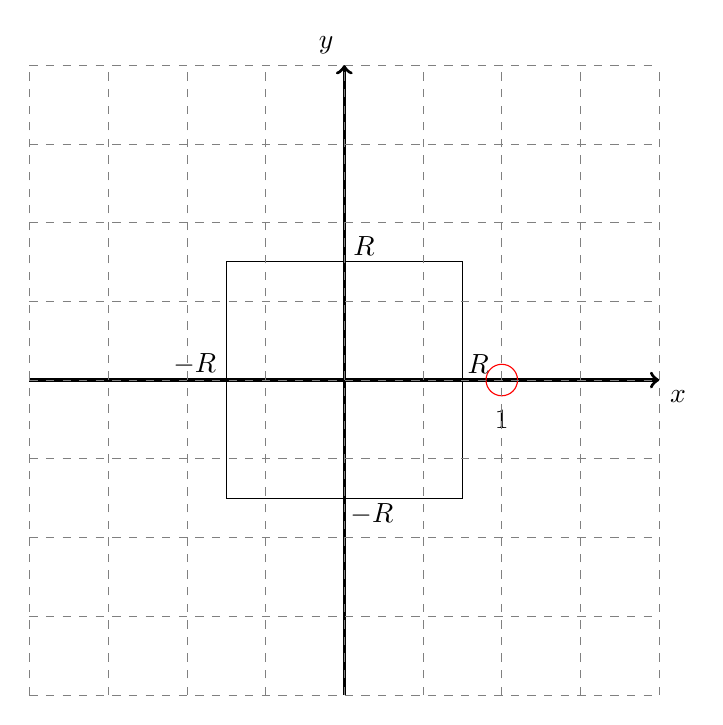
\begin{tikzpicture}
\draw[very thick,->] (-4,0) -- (4,0) node[anchor=north west] {$x$};
\draw[very thick,->] (0,-4) -- (0,4) node[anchor=south east] {$y$};
\draw (-1.5,1.5) -- (-1.5,-1.5) -- (1.5,-1.5) -- (1.5,1.5)--(-1.5,1.5); 
\draw[red] (2,0) circle (2mm) ;

\node at (2,-0.5) {1};
\node at (-1.9,0.2) {$-R$};
\node at (1.7,0.2) {$R$};
\node at (0.35,-1.7) {$-R$};
\node at (0.25,1.7) {$R$};



\draw[step=1cm,gray,dashed,very thin] (-4,-4) grid (4,4);
\end{tikzpicture}

Η $f$ είναι αναλυτική στο εσωτερικό και πάνω  στην απλή κλειστή τμηματικά λεία καμπύλη $C_{R}$. Άρα $Ι=0$.

\begin{itemize}
\item Όταν έχουμε $R=1$ :
\end{itemize}

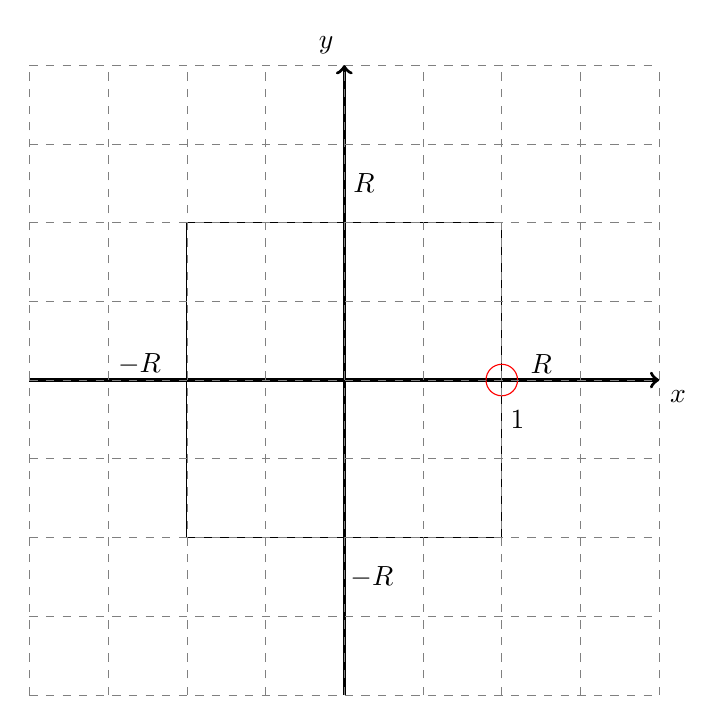
\begin{tikzpicture}
\draw[very thick,->] (-4,0) -- (4,0) node[anchor=north west] {$x$};
\draw[very thick,->] (0,-4) -- (0,4) node[anchor=south east] {$y$};
\draw (-2,2) -- (-2,-2) -- (2,-2) -- (2,2)--(-2,2); 
\draw[red] (2,0) circle (2mm) ;

\node at (2.2,-0.5) {1};
\node at (-2.6,0.2) {$-R$};
\node at (2.5,0.2) {$R$};
\node at (0.35,-2.5) {$-R$};
\node at (0.25,2.5) {$R$};



\draw[step=1cm,gray,dashed,very thin] (-4,-4) grid (4,4);
\end{tikzpicture}
\newline
Η $f$ είναι αναλυτική στο εσωτερικό και πάνω  στην απλή κλειστή τμηματικά λεία καμπύλη $C_{R}$ με εξαίρεση το σημείο $z=1$ το οποίο βρίσκεται πάνω στη καμπύλη. Άρα $Ι=\pi i Res(f,1)= \pi i $.

Όπου :$$Res(f,1) =\lim_{z\to 1}\left[ (z-1)f(z)  \right]=
\lim_{z\to 1}\left[ \frac{(z-1) {\sin^{2}(z-1)}}{(z-1)^{3}}  \right]=
$$ 
$$=\lim_{z\to 1}\left[ \frac{{\sin^{2}(z-1)}}{(z-1)^{2}}  \right]
=\lim_{z\to 1} \left[ \frac{{\sin(z-1)}}{z-1}  \right]^{2}=1$$

Αφού

$$ \lim_{z\to 1} \left[\frac{{\sin(z-1)}}{z-1}\right] \overset{\mathrm{De L'Hospital}}{=\joinrel=\joinrel=\joinrel=\joinrel=\joinrel=\joinrel=} \lim_{z\to 1} \left[ \frac{{\cos(z-1)}}{1}  \right]=1 $$


\begin{itemize}
\item Όταν έχουμε $R>1$ :
\end{itemize}

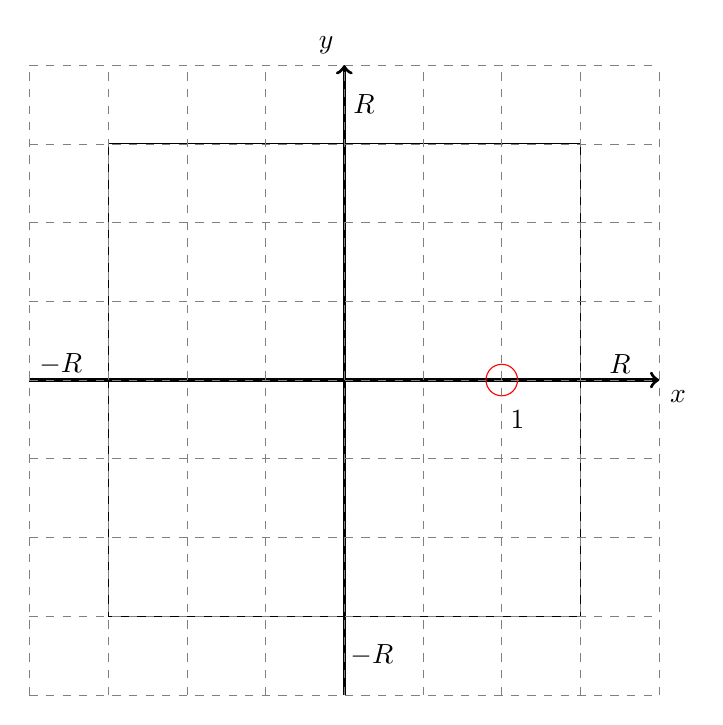
\begin{tikzpicture}
\draw[very thick,->] (-4,0) -- (4,0) node[anchor=north west] {$x$};
\draw[very thick,->] (0,-4) -- (0,4) node[anchor=south east] {$y$};
\draw (-3,3) -- (-3,-3) -- (3,-3) -- (3,3)--(-3,3); 
\draw[red] (2,0) circle (2mm) ;

\node at (2.2,-0.5) {1};
\node at (-3.6,0.2) {$-R$};
\node at (3.5,0.2) {$R$};
\node at (0.35,-3.5) {$-R$};
\node at (0.25,3.5) {$R$};



\draw[step=1cm,gray,dashed,very thin] (-4,-4) grid (4,4);
\end{tikzpicture}
\newline
Η $f$ είναι αναλυτική στο εσωτερικό και πάνω  στην απλή κλειστή τμηματικά λεία καμπύλη $C_{R}$ με εξαίρεση το σημείο $z=1$ το οποίο βρίσκεται στο εσωτερικό της καμπύλης. Άρα $Ι= 2 \pi i Res(f,1)= 2 \pi i $.

Όπου :$$Res(f,1) =\lim_{z\to 1}\left[ (z-1)f(z)  \right]=
\lim_{z\to 1}\left[ \frac{(z-1) {\sin^{2}(z-1)}}{(z-1)^{3}}  \right]=
$$ 
$$=\lim_{z\to 1}\left[ \frac{{\sin^{2}(z-1)}}{(z-1)^{2}}  \right]
=\lim_{z\to 1} \left[ \frac{{\sin(z-1)}}{z-1}  \right]^{2}=1$$

Αφού

$$ \lim_{z\to 1} \left[\frac{{\sin(z-1)}}{z-1}\right] \overset{\mathrm{De L'Hospital}}{=\joinrel=\joinrel=\joinrel=\joinrel=\joinrel=\joinrel=} \lim_{z\to 1} \left[ \frac{{\cos(z-1)}}{1}  \right]=1 $$


\newpage
 \subsection{Άσκηση 3}

$$I= \int_{-\infty}^{+\infty} \frac{dx}{(x+2)(x^2+1)^2}$$
\\ Λύνουμε

$$ (z+2)(z^2+1)^2=0 \Rightarrow$$ 
$
z+2=0\Rightarrow z=-2 \quad $ ή $ \quad$ 
\\
$ z^2+1=0\Rightarrow (z+i)(z-i)=0 \Rightarrow z=i \quad$ ή $ \quad z=-i$
\\
\\
Θέτουμε $ f(z)=\frac{1}{(z+2)(z^2+1)^2},z\in\mathbb{C}-\{-i,i,-2\} $
\\  \\
Άρα έχουμε δύο πόλους δεύτερης τάξης, έναν στο άνω και έναν στο κάτω ημιεπίπεδο και έναν πόλο πρώτης τάξης πάνω στον πραγματικό άξονα.

$$ \lim_{z \to \infty } zf(z)=\lim_{z \to \infty } \frac{z}{(z+2)(z^2+1)^2}=
\lim_{z \to \infty } \frac{z}{z\left(1+\frac{2}{z}\right)(z^2+1)^2}=
\lim_{z \to \infty } \frac{1}{\left(1+\frac{2}{z}\right)(z^2+1)^2}=0$$

Επομένως $$ Ι= 2 \pi i Res(f,i)+ \pi i Res(f,-2)\quad (1) $$
$$  Res(f,-2)=\lim_{z\to -2}\frac{z+2}{(z+2)(z^2+1)^2}=\lim_{z\to -2}\frac{1}{(z^2+1)^2}=\frac{1}{25}$$

$$ Res(f,i)=\lim_{z\to i} \left[ \frac{(z-i)^2}{(z+2)(z+i)^2(z-i)^2} \right]^{'}= \lim_{z\to i} \left[-\frac{(z+i)^2+2(z+2)(z+i)}{(z+2)^2(z+i)^4}\right]=$$
$$= -\frac{(2i)^2+2(2+i)(2i)}{(2+i)^2(2i)^4}= -\frac{-4+4i(2+i)}{(3+4i)(2i)^4}= \frac{8-8i}{(3+4i)(2i)(-8i)}=\frac{i(1-i)(3-4i)}{(9+16)(2i)}=$$
$$=\frac{(1+i)(3-4i)}{(2i)25}=\frac{7-i}{(2i)25} $$
\\
Άρα η $(1)$ γίνεται:
\\
$$ Ι=2\pi i \left[ \frac{7-i}{(2i)25} \right] + \pi i \left[ \frac{1}{25} \right] = \frac{ 7\pi -\pi i}{25} + \frac{ \pi i}{25}= \frac{ 7\pi}{25}$$
\\
Άρα $$ \int_{-\infty}^{+\infty} \frac{dx}{(x+2)(x^2+1)^2}=\frac{ 7\pi}{25} $$

 

\newpage 
\part{Εφαρμοσμένα Μαθηματικά Σεπτέμβριος 2016}

  

\maketitle
\newpage
 


 \section{Θέματα Ατρέα}

 \subsection{Άσκηση 1}

Η $g$ είναι αναλυτική στο $D\subseteq \mathbb{C}$
\\
$$ g(z)=g(x+yi)=u(x,y)+iv(x,y) $$
\\
Από τις εξισώσεις $Cauchy-Riemann$ έχουμε
\\
\[
\spalignsys {u_x=v_y;u_y=-v_x} \Rightarrow    
\spalignsys {u_{xx}=v_{yx} \quad (1);u_{yy}=-v_{xy} \quad (2) }
\]

$$(1),(2)\overset{(+)}{\Rightarrow} u_{xx}+u_{yy}=v_{yx}-v_{xy} \Rightarrow u_{xx}+u_{yy}=v_{xy}-v_{xy} \Rightarrow u_{xx}+u_{yy}=0 $$
αφού η $ v(x,y) $ έχει συνεχείς μερικές παραγώγους, $v_{xy}=v_{yx} $
\\ \\
Άρα η $f$ αρμονική στο $D$


 \subsection{Άσκηση 2}

$ P(z)=ae^{z}+b\sin(z), \quad a,b\in\mathbb{C} $\\ \\
$ P'(z)=ae^{z}+b\cos(z) $\\
$ P''(z)=ae^{z}-b\sin(z) ,\quad P''(0)=a$\\
$ P^{(3)}(z)=ae^{z}-b\cos(z),\quad P^{(3)}(0)=a-b $\\

Θεωρούμε την $g(z)=(z+1)P(z),z\in \mathbb{C}$
\\ \\
$ g'(z)=P(z)+(z+1)P'(z) ,\quad g(0)=a $\\
$ g''(z)=2P'(z)+(z+1)P''(z) $\\
$ g^{(3)}(z)=3P''(z)+(z+1)P^{3}(z), \quad g^{(3)}(0)=4a-b $\\


Το σημείο $ z=0 \quad$ βρίσκεται εντός της καμπύλης $\gamma : |z|=2$
\\
Επομένως, από τον ολοκληρωτικό τύπο του $Cauchy$ για παραγώγους έχουμε:
$$ g(0)=\frac{1}{2\pi i} \int_\gamma \frac{g(z)}{z}=\frac{1}{2\pi i} \int_\gamma \frac{(z+1)P(z)}{z}=\frac{2}{2\pi i}=-\frac{i}{\pi} $$

$$ g^{(3)}(0)=\frac{3!}{2\pi i} \int_\gamma \frac{g(z)}{z^4}=\frac{6}{2\pi i} \int_\gamma \frac{(z+1)P(z)}{z^4}=\frac{9i}{\pi i}=\frac{9}{\pi} $$
\\
\[
\spalignsys {a=-\frac{i}{\pi}; ;4a-b=\frac{9}{\pi}}
\Rightarrow
\spalignsys { a=-\frac{i}{\pi}; ;-4i-b\pi= 9}
\Rightarrow
\spalignsys {a=-\frac{i}{\pi}; ;b=-\frac{9+4i}{\pi} }
\]

 \subsection{Άσκηση 3}

$$ I=\oint_{\gamma}\overline{z}^{^6}(z^5+2z)dz, \quad \gamma:|z|=2 $$

Θεωρούμε την $ f(z)=\overline{z}^{^6}(z^5+2z),\quad z\in\mathbb{C}$
\\ \\
Παραμετροποίση κύκλου $\gamma$:
$$ \gamma(t)=2e^{it},\quad t\in[0,2\pi] $$
$$ \qquad \gamma'(t)=2ie^{it}  $$

$$ Ι=\oint_{\gamma}f(z)dz=\oint_{\gamma}f(\gamma(t))\gamma'(t)dt= \int_{0}^{2\pi} (2^6e^{-6it})(2^5e^{5it}+4e^{it})(2ie^{it}) dt= $$

$$ =\int_{0}^{2\pi} (2^12 +2^9 e^{-4it}) dt = 2^9\int_{0}^{2\pi} (8 +  e^{-4it}) dt =  2^9 \left[ 8t - \frac { e^{-4it} }{4i} \right]_{0}^{2\pi}= 2^9\cdot 16\pi=8192\pi $$


\newpage



 \subsection{Άσκηση 4}
$$I= \int_{-\infty}^{+\infty} \frac{dx}{(x-1)(x^2+1)^2}$$
\\ Λύνουμε

$$ (z-1)(z^2+1)^2=0 \Rightarrow$$ 
$
z-1=0\Rightarrow z=1 \quad $ ή $ \quad$ 
\\
$ (z^2+1)^2=0\Rightarrow (z+i)^2(z-i)^2=0 \Rightarrow z=i \quad$ ή $ \quad z=-i$
\\
\\
Θέτουμε $ f(z)=\frac{1}{(z-1)(z^2+1)^2},z\in\mathbb{C}-\{-i,i,1\} $
\\ \\
Άρα έχουμε δύο πόλους δεύτερης τάξης, έναν στο άνω, έναν στο κάτω ημιεπίπεδο και έναν πόλο πρώτης τάξης πάνω στον πραγματικό άξονα.

$$ \lim_{z \to \infty } zf(z)=\lim_{z \to \infty } \frac{z}{(z-1)(z^2+1)^2}=
\lim_{z \to \infty } \frac{z}{z\left(1-\frac{1}{z}\right)(z^2+1)^2}=
\lim_{z \to \infty } \frac{1}{\left(1-\frac{1}{z}\right)(z^2+1)^2}=0$$

Επομένως $$ Ι= 2 \pi i Res(f,i)+ \pi i Res(f,1)\quad (1) $$

$$  Res(f,1)=\lim_{z\to 1}\frac{z-1}{(z-1)(z^2+1)^2}=\lim_{z\to 1}\frac{1}{(z^2+1)^2}=\frac{1}{4}$$

$$ Res(f,i)=\lim_{z\to i} \left[ \frac{(z-i)^2}{(z-1)(z+i)^2(z-i)^2} \right]^{'}= \lim_{z\to i} \left[-\frac{(z+i)^2+2(z-1)(z+i)}{(z-1)^2(z+i)^4}\right]=$$

$$= -\frac{(2i)^2+2(-1+i)(2i)}{(-1+i)^2(2i)^4}= \frac{4(-1-i-1 )}{16(2i)}= -\frac{2+i}{4(2i)} $$

Άρα η $(1)$ γίνεται:
\\
$$ Ι=2\pi i \left[ -\frac{2+i}{4(2i)} \right] + \pi i \left( \frac{1}{4} \right) = \frac{ -2\pi -\pi i}{4} + \frac{ \pi i}{4}= -\frac{ \pi}{2}$$

Άρα $$ \int_{-\infty}^{+\infty} \frac{dx}{(x-1)(x^2+1)^2}=-\frac{ \pi}{2} $$
\newpage

 \section{Θέματα Κεχαγιά}

 \subsection{Άσκηση 1}

Θέτουμε $ w=z+\frac{100}{z}$

$$ |z|+\frac{100}{|z|}=20 \Rightarrow |z|^2 -20|z|+100=0 \Rightarrow (|z|-10)^2=0\Rightarrow |z|=10$$
$$|z|=10 \Rightarrow |z|^2=100 \Rightarrow z\overline{z}=100 \Rightarrow \overline{z}=\frac{100}{z} \quad (1)$$

Λόγω της $(1)$ έχουμε: $w=z+\overline{z}=2Re(z)\in\mathbb{R}$
\\ \\
Άρα $Im\left( z+\frac{100}{z} \right)=0$

 \subsection{Άσκηση 2}

$$(z+2)^3=z^3\overset{z\neq0}{\Longrightarrow} \left( \frac{z+2}{z} \right)^3=1 \Rightarrow \left( 1 + \frac{2}{z} \right)=\sqrt[3]{|1|}e^{i \frac{2\kappa \pi}{3}},\quad \kappa = 0,1,2 $$

Άρα:
\\ \\
$ \bullet \quad 1 + \frac{2}{z}=1\Rightarrow 2=0 ,\quad$
αδύνατο

$$ \bullet \quad 1 + \frac{2}{z}= e^{i \frac{2 \pi}{3}} \Rightarrow \frac{2}{z}= -\frac{1}{2} + \frac{\sqrt{3}}{2} - 1 \Rightarrow z=\frac{4}{-3+i \sqrt{3}} \Rightarrow $$
$$ \Rightarrow z=\frac{4(-3-i \sqrt{3})}{12} \Rightarrow z=-\left(1+i \frac{\sqrt{3}}{3}\right)  $$

$$ \bullet \quad 1 + \frac{2}{z}= e^{i \frac{4 \pi}{3}} \Rightarrow \frac{2}{z}= -\frac{1}{2} - \frac{\sqrt{3}}{2} - 1 \Rightarrow z=-\frac{4}{3+i \sqrt{3}} \Rightarrow $$
$$ \Rightarrow z=-\frac{4(3-i \sqrt{3})}{12} \Rightarrow z=-\left(1-i \frac{\sqrt{3}}{3}\right)  $$

\newpage

 \subsection{Άσκηση 3}

$$ i^i=e^{i \log(i)}=e^{i (\ln|i| + i (\pi + 2\kappa \pi) )}=e^{-\pi(2\kappa+1)},\quad\kappa \in \mathbb{Z} $$

 \subsection{Άσκηση 4}
$$
\sum_{n=0}^{\infty} r^n \sin(a n)=\sum_{n=0}^{\infty} r^n \frac{e^{i (a n)}-e^{-i (a n)}}{2i}=$$

$$ =\frac{1}{2i}\sum_{n=0}^{\infty} (r e^ { i a })^n - \frac{1}{2i}\sum_{n=0}^{\infty}(r e^ { -i a })^n\overset{\mathrm{0<r<1}}{ =\joinrel=\joinrel=\joinrel=\joinrel=}\frac{1}{2i} \left ( \frac{1}{1-re^{ia}}-\frac{1}{1-re^{-ia}}\right)=$$

$$ = \frac{1}{2i} \left [ \frac{1-re^{-ia}-(1-re^{ia})}{(1-re^{ia})(1-re^{-ia})} \right] =\frac{1}{2i} \left [ \frac{re^{ia}-re^{-ia}}{1-re^{ia}-re^{-ia}+r^2} \right] = $$

$$ = \frac{e^{ia}-e^{-ia}}{2i} \left [ \frac{r}{1+r^2-2r\left( \frac {e^{ia}-e^{-ia}}{2}\right)} \right] =  \frac{r \sin(a)}{1+r^2-2r\cos(a)} $$

\newpage
 \subsection{Άσκηση 5}

$$ f(z)=\frac{1}{z^2+4}=\frac{1}{(z-2i)(z+2i)},z\in\mathbb{C}-\{-2i,2i\} $$ 
\\
$ Laurent $ γύρω από το $ z_0=1 $
\\ \\
Έστω $A,B\in \mathbb{C}$  τέτοια ώστε:
$$ \frac{1}{(z-2i)(z+2i)}= \frac{A}{z-2i}+\frac{B}{z+2i} \Rightarrow
A(z+2i)+B(z-2i)=1 \Rightarrow (A+B)z+2i(A-B)=1 \Rightarrow $$

\[
\Rightarrow
\spalignsys{A+B=0; ;2i(A-B)=1}
\Rightarrow
\spalignsys{B=-A; ;2A=\frac{1}{2i}}
\Rightarrow
\spalignsys{B=-A; ;A=\frac{1}{4i}}
\Rightarrow
\spalignsys{B=-\frac{1}{4i}; ;A=\frac{1}{4i}}
\]
\\ \\
Άρα

$$ f(z)=\frac{1}{z^2+4}= \frac{1}{4i}\left( \frac{1}{z-2i} - \frac{1}{z+2i} \right) = \frac{1}{4i}\left[ \frac{1}{(z-1)+(1-2i)} - \frac{1}{(z-1)+(1+2i)} \right] =$$

$$
=
\frac{1}{4i}\left[\frac{1}{1-2i} \left( \frac{1}{1+\frac{z-1}{1-2i} } \right) -
\frac{1}{1+2i} \left(  \frac{1}{1+\frac{z-1}{1+2i}}\right)\right]=
$$
$$
=\frac{1}{4i}\sum_{n=0}^{\infty}(-1)^n
\frac{(z-1)^n}{(1-2i)^{n+1}}-
\frac{1}{4i}\sum_{n=0}^{\infty}(-1)^n
\frac{(z-1)^n}{(1+2i)^{n+1}}=\frac{1}{5}-\frac{2(z-1)}{25}-\frac{1(z-1)^2}{125}+\frac{12(z-1)^3}{625}-\ldots
$$
για $|z-2i|<|1\pm2i|=\sqrt{5}$




$$ f(z)=\frac{1}{z^2+4}= \frac{1}{4i}\left( \frac{1}{z-2i} - \frac{1}{z+2i} \right) = \frac{1}{4i}\left[ \frac{1}{(z-1)+(1-2i)} - \frac{1}{(z-1)+(1+2i)} \right] =$$

$$
=
\frac{1}{4i}\left[\frac{1}{z-1} \left( \frac{1}{1+\frac{1-2i}{z-1} } \right) -
\frac{1}{z-1} \left( \frac{1}{1+\frac{1+2i}{z-1} }\right)
\right]=
$$
$$
=\frac{1}{4i}\sum_{n=0}^{\infty}(-1)^n
\frac{(1-2i)^n}{(z-1)^{n+1}}-
\frac{1}{4i}\sum_{n=0}^{\infty}(-1)^n
\frac{(1+2i)^n}{(z-1)^{n+1}}=\frac{1}{(z-1)^2}-\frac{2}{(z-1)^3}+\ldots
$$
για $|z-2i|>|1\pm2i|=\sqrt{5}$

\newpage
 


\newpage \part{Εφαρμοσμένα Μαθηματικά Φεβρουάριος 2016}

  

\maketitle
\newpage
 



 \section{Θέματα Ατρέα}

 \subsection{Άσκηση 1}

Η $g$ είναι αναλυτική στο $Α\subseteq \mathbb{C}$ και $Im\left(g(z)\right)=d, \quad d \in\mathbb{R}$
\\
$$ g(z)=g(x+yi)=u(x,y)+iv(x,y)=u(x,y)+id $$
\\
Από τις εξισώσεις $Cauchy-Riemann$ έχουμε
\\
\[
\spalignsys {u_x=v_y;u_y=-v_x} \Rightarrow    
\spalignsys {u_x=0=v_y;u_y=0=v_x }
\]
\\
Άρα $\quad f'(z)=f_x=u_x+iv_x=0 $
\\ δηλαδή $$ f(z)=c \quad ,c \in \mathbb{C} $$

 \subsection{Άσκηση 2}

$$I = \oint_{C_R} \frac{dz}{z^2(z+4i)}, \quad C_R:|z-3i|=R $$

Θεωρούμε την  $f(z)=\frac{1}{z^2(z+4i)}, z\in\mathbb{C}-\{0,-4i\}$ .

\begin{itemize}
\item Όταν έχουμε $R<3$ :
\end{itemize}

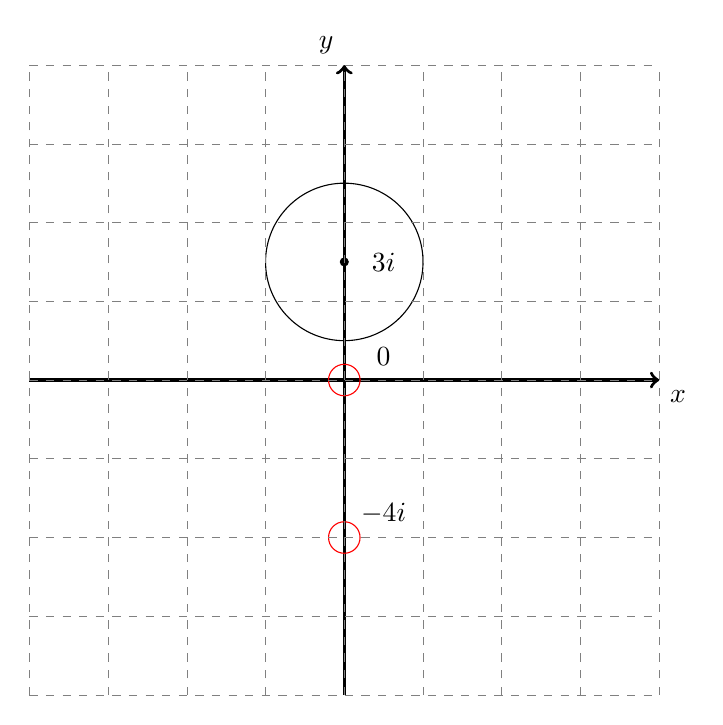
\begin{tikzpicture}
\draw[very thick,->] (-4,0) -- (4,0) node[anchor=north west] {$x$};
\draw[very thick,->] (0,-4) -- (0,4) node[anchor=south east] {$y$};
\draw (0,1.5) circle (1cm);
\filldraw[black] (0,1.5) circle (0.5mm) ;

\draw[red] (0,0) circle (2mm) ;
\draw[red] (0,-2) circle (2mm) ;


\node at (0.5,1.5) {$3i$};
\node at (0.5,0.3) {$0$};
\node at (0.5,-1.7) {$-4i$};


\draw[step=1cm,gray,dashed,very thin] (-4,-4) grid (4,4);
\end{tikzpicture}

Η $f$ είναι αναλυτική στο εσωτερικό και πάνω  στην απλή κλειστή τμηματικά λεία καμπύλη $C_{R}$. Άρα $Ι=0$.

\begin{itemize}
\item Όταν έχουμε $3<R<7$ :
\end{itemize}

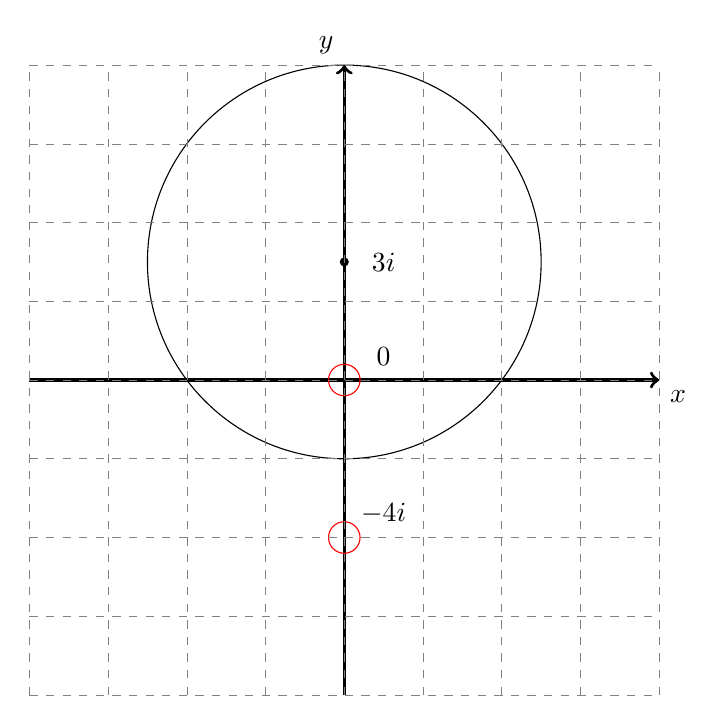
\begin{tikzpicture}
\draw[very thick,->] (-4,0) -- (4,0) node[anchor=north west] {$x$};
\draw[very thick,->] (0,-4) -- (0,4) node[anchor=south east] {$y$};
\draw (0,1.5) circle (2.5cm);
\filldraw[black] (0,1.5) circle (0.5mm) ;

\draw[red] (0,0) circle (2mm) ;
\draw[red] (0,-2) circle (2mm) ;


\node at (0.5,1.5) {$3i$};
\node at (0.5,0.3) {$0$};
\node at (0.5,-1.7) {$-4i$};


\draw[step=1cm,gray,dashed,very thin] (-4,-4) grid (4,4);
\end{tikzpicture}
\newline
Η $f$ είναι αναλυτική στο εσωτερικό και πάνω  στην απλή κλειστή τμηματικά λεία καμπύλη $C_R$ με εξαίρεση το σημείο $z=0$ το οποίο βρίσκεται στο εσωτερικό της. Άρα $Ι=2 \pi i Res(f,0)= \frac{\pi i}{8} $.
\\
Όπου :
$$ Res(f,0)= \lim_{z\to 0} \left[ \frac{z^2}{z^2(z+4i)} \right]'= \lim_{z\to 0} \left( \frac{1}{z+4i} \right)' = \lim_{z\to 0} - \frac{1}{(z+4i)^2} =\frac{1}{16} $$

\begin{itemize}
\item Όταν έχουμε $R>7$ :
\end{itemize}

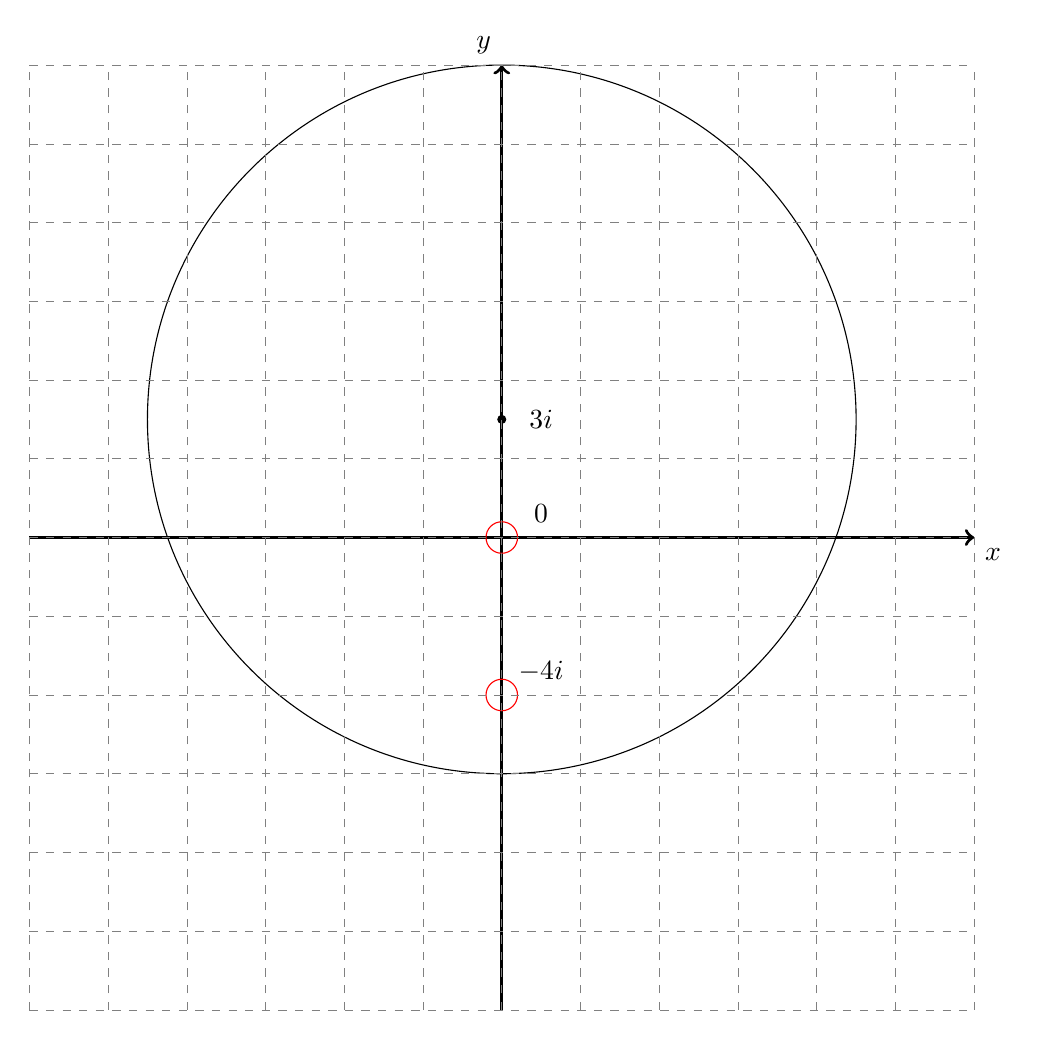
\begin{tikzpicture}
\draw[very thick,->] (-6,0) -- (6,0) node[anchor=north west] {$x$};
\draw[very thick,->] (0,-6) -- (0,6) node[anchor=south east] {$y$};
\draw (0,1.5) circle (4.5cm);
\filldraw[black] (0,1.5) circle (0.5mm) ;

\draw[red] (0,0) circle (2mm) ;
\draw[red] (0,-2) circle (2mm) ;


\node at (0.5,1.5) {$3i$};
\node at (0.5,0.3) {$0$};
\node at (0.5,-1.7) {$-4i$};


\draw[step=1cm,gray,dashed,very thin] (-6,-6) grid (6,6);
\end{tikzpicture}
\newline
Η $f$ είναι αναλυτική στο εσωτερικό και πάνω  στην απλή κλειστή τμηματικά λεία καμπύλη $C_{R}$ με εξαίρεση τα σημεία $z=0$ και $ z=-4i$ τα οποία βρίσκονται στο εσωτερικό της. Άρα $Ι= 2 \pi i \left( Res(f,0)+ Res(f,-4i) \right)= 0 $.
\\
Όπου :$$ Res(f,0)= \lim_{z\to 0} \left[ \frac{z^2}{z^2(z+4i)} \right]'= \lim_{z\to 0} \left( \frac{1}{z+4i} \right)' = \lim_{z\to 0} - \frac{1}{(z+4i)^2} =\frac{1}{16} $$

$$ Res(f,-4i)= \lim_{z\to -4i}  \frac{z+4i}{z^2(z+4i)} = \lim_{z\to -4i}  \frac{1}{z^2} = -\frac{1}{16} $$
\\
 \subsection{Άσκηση 3}
$f(z)=(3z-1)\sin\left(\frac{3}{z-1}\right)=[3(z-1)+2]\sin\left(\frac{3}{z-1}\right)$
όμως
$$\sin\left(\frac{3}{z-1}\right)=\sum_{n=1}^{\infty} \left[ \frac{(-1)^{n+1}}{(2n-1)!}\left(\frac{3}{z-1}\right)^{n+1} \right] $$
άρα
$$ f(z)= [3(z-1)+2] \left[ \frac{3}{z-1} - \left(\frac{3}{z-1}\right)^3\frac{1}{3!} + \left(\frac{3}{z-1}\right)^5\frac{1}{5!} - ... \right] \Rightarrow $$
$$\Rightarrow f(z)=3\cdot3-\frac{3\cdot3^3}{(z-1)^2 3!} + \frac{3\cdot3^5}{(z-1)^4 5!}-...+\frac{6}{z-1}- \frac{2\cdot3^3}{(z-1)^3 3!}+ \frac{2\cdot3^5}{(z-1)^5 5!}-...$$
\\
Κι αφού ο συντελεστής του όρου $\frac{1}{z-1}$ είναι το $6$ θα έχουμε:
$$ Res(f,1)=6 $$



 \subsection{Άσκηση 4}
$$I= \int_{-\infty}^{+\infty} \frac{dx}{(x-2)(x^2+4)}$$
\\ Λύνουμε

$$ (z-2)(z^2+4)=0 \Rightarrow$$ 
$
z-2=0\Rightarrow z=2 \quad $ ή $ \quad$ 
\\
$ z^2+4=0\Rightarrow (z+2i)(z-2i)=0 \Rightarrow z=2i \quad$ ή $ \quad z=-2i$
\\
\\
Θέτουμε $ f(z)=\frac{1}{(z-2)(z^2+4)},z\in\mathbb{C}-\{-2i,2i,2\} $
\\
Άρα έχουμε τρεις πόλους πρώτης τάξης, έναν στο άνω, έναν στο κάτω ημιεπίπεδο και έναν πάνω στον πραγματικό άξονα.

$$ \lim_{z \to \infty } zf(z)=\lim_{z \to \infty } \frac{z}{(z-2)(z^2+4)}=
\lim_{z \to \infty } \frac{z}{z\left(1-\frac{2}{z}\right)(z^2+4)}=
\lim_{z \to \infty } \frac{1}{\left(1-\frac{2}{z}\right)(z^2+4)}=0$$

Επομένως $$ Ι= 2 \pi i Res(f,2i)+ \pi i Res(f,2)\quad (1) $$

$$  Res(f,2)=\lim_{z\to 2}\frac{z-2}{(z-2)(z^2+4)}=\lim_{z\to 2}\frac{1}{(z^2+4)}=\frac{1}{8}$$

$$ Res(f,2i)=\lim_{z\to 2i} \left[ \frac{(z-2i)}{(z-2)(z+2i)(z-2i)} \right]= \lim_{z\to 2i} \left[ \frac{1}{(z-2)(z+2i)} \right]=  \frac{1}{(2i-2)(4i)}= $$
$$ =\frac{1}{-(4-4i)(2i)}= \frac{(4+4i)}{-(16+16)(2i)}= \frac{-(1+i)}{8(2i)} $$
\\
Άρα η $(1)$ γίνεται:
\\
$$ Ι=2\pi i \left[ \frac{-1-i}{(2i)8} \right] + \pi i \left( \frac{1}{8} \right) = \frac{ -\pi -\pi i}{8} + \frac{ \pi i}{8}= -\frac{ \pi}{8}$$
\\
Άρα $$ \int_{-\infty}^{+\infty} \frac{dx}{(x-2)(x^2+4)}= -\frac{\pi}{8} $$
\newpage

 \section{Θέματα Κεχαγιά}

 \subsection{Άσκηση 1}

$$ \spalignsys{ z=\overline{z}|z|; \overline{z}=z|z|} \Rightarrow z=( z|z|)|z| \Rightarrow z=z|z|^2 \Rightarrow z(1-|z|^2)=0\Rightarrow $$
\\
$\Rightarrow z=0 \quad$ ή $\quad |z|=1 $
\\
Αν $|z|=1$ τότε:

$$ z=\overline{z}|z| \Rightarrow z=\overline{z} \Rightarrow z\in\mathbb{R}$$
και αφού $|z|=1$, $z=-1$ ή $z=1$
\\
Επομένως οι λύσεις της εξίσωσης είναι:
$$ z=-1 \quad ,\quad z=0 \quad,\quad z=1$$


 \subsection{Άσκηση 2}
Θέτουμε $ w=z+\frac{100}{z}$

$$ |z|+\frac{100}{|z|}=20 \Rightarrow |z|^2 -20|z|+100=0 \Rightarrow (|z|-10)^2=0\Rightarrow |z|=10$$
$$|z|=10 \Rightarrow |z|^2=100 \Rightarrow z\overline{z}=100 \Rightarrow \overline{z}=\frac{100}{z} \quad (1)$$

Λόγω της $(1)$ έχουμε: $w=z+\overline{z}=2Re(z)\in\mathbb{R}$

\newpage

 \subsection{Άσκηση 3}

$$ \cos\left(\frac{\pi}{6}\right)+\cos\left(\frac{3\pi}{6}\right)+...+\cos\left(\frac{9\pi}{6}\right)= 
\sum_{n=0}^{4} \cos\left(\frac{(2n+1)\pi}{6}\right)=\sum_{n=0}^{4} \frac{e^{i\frac{(2n+1)\pi}{6}}+e^{-i\frac{(2n+1)\pi}{6}}}{2}=$$

$$ =\frac{e^ {i \frac{\pi}{6} }}{2}\sum_{n=0}^{4} { e^ {i \frac{n\pi}{3} } } + \frac{e^ {-i \frac{\pi}{6} }}{2}\sum_{n=0}^{4} { e^ {-i \frac{n\pi}{3} }} 
=\frac{e^ {i \frac{\pi}{6} }}{2} \left[ \frac{ { \left( e^ {i \frac{\pi}{3} }\right) }^4-1}{ { e^ {i \frac{\pi}{3} } -1}} \right] + \frac{e^ {-i \frac{\pi}{6} }}{2} \left[ \frac{ { \left( e^ {-i \frac{\pi}{3} }\right) }^4-1}{ { e^ {-i \frac{\pi}{3} } -1}} \right]= $$

$$=\frac{1}{2} \left( \frac{\sqrt{3}+i}{2} \right) \left( \frac{-\frac{1+i\sqrt{3}}{2}-1}{\frac{1+i\sqrt{3}}{2}-1} \right) + \frac{1}{2} \left( \frac{\sqrt{3}-i}{2} \right) \left( \frac{\frac{-1+i\sqrt{3}}{2}-1}{\frac{1-i\sqrt{3}}{2}-1} \right)=  $$

$$= -\left( \frac{\sqrt{3}+i}{4} \right)\left( \frac{1+i\sqrt{3}+2}{1+i\sqrt{3}-2} \right) +
\left( \frac{\sqrt{3}-i}{4} \right)\left( \frac{-1+i\sqrt{3}-2}{1-i\sqrt{3}-2} \right)= $$

$$ = \left( \frac{\sqrt{3}+i}{4} \right)\left( \frac{3+i\sqrt{3}}{1-i\sqrt{3}} \right) +
\left( \frac{\sqrt{3}-i}{4} \right)\left( \frac{-3+i\sqrt{3}}{-1-i\sqrt{3}} \right)= $$

$$ = i\left( \frac{1-i\sqrt{3}}{4} \right)\left( \frac{3+i\sqrt{3}}{1-i\sqrt{3}} \right) + i
\left( \frac{-1-i\sqrt{3}}{4} \right)\left( \frac{-3+i\sqrt{3}}{-1-i\sqrt{3}} \right)= $$

$$ = \left( \frac{3i-\sqrt{3}}{4} \right) + 
\left( \frac{-\sqrt{3}-3i}{4} \right) = -\frac{\sqrt{3}}{2} $$
\newpage
 \subsection{Άσκηση 4}

$$ f(z)=\frac{1}{z^2-1}=\frac{1}{(z+1)(z-1)}=\frac{1}{2}\left( \frac{1}{z-1}\right)-\frac{1}{2}\left(\frac{1}{z+1}\right)=\frac{1}{2}\left(\frac{1}{z-1}\right)-\frac{1}{2}\left[ \frac{1}{(z-1)+2}\right] $$

$$\bullet \quad 
f(z)=\frac{1}{2}\left(\frac{1}{z-1}\right) -\frac{1}{4}\left( \frac{1}{1+\frac{z-1}{2}} \right) =
\frac{1}{2}\left( \frac{1}{z-1}\right)-\frac{1}{4}
\sum_{n=0}^{\infty}(-1)^n\frac{(z-1)^n}{2^n}=
$$
$$=
\frac{1}{2(z-1)}-\frac{1}{4}+\frac{z-1}{8}-
\frac{(z-1)^2}{16}+\frac{(z-1)^3}{32}-\ldots \quad ,\quad |z-1|<2
$$

$$\bullet \quad
f(z)=\frac{1}{2}\left(\frac{1}{z-1}\right)-\frac{1}{2(z-1)}\left( \frac{1}{1+\frac{2}{z-1}}\right) =
\frac{1}{2}\left(\frac{1}{z-1}\right) -\frac{1}{2}
\sum_{n=0}^{\infty}(-1)^n\frac{2^n}{(z-1)^n}=
$$$$
=-\frac{1}{2}+\frac{3}{2(z-1)}-\frac{2}{(z-1)^2}+\frac{4}{(z-1)^3}-\ldots \quad,\quad |z-1|>2
$$

\newpage
 \subsection{Άσκηση 5}

$$ u(x,y)=\frac{\cos(x)\cosh(y)x}{x^2+y^2}-\frac{\sin(x)\sinh(y)y}{x^2+y^2} $$
με $ f(z)=f(x+yi)=u(x,y)+iv(x,y) $
\\ \\
Έστω $g:\mathbb{C}\to\mathbb{C}$ και $ h:\mathbb{C}-\{0\}\to\mathbb{C}$ τέτοιες ώστε $f(z)=g(z)h(z)\Leftrightarrow $

$$ \Leftrightarrow f(z)=[Re(g(z))+iIm(g(z))][Re(h(z))+iIm(h(z))] \Leftrightarrow $$

$$\Leftrightarrow \spalignsys{Re(f(z))=Re(g(z))Re(h(z))-Im(g(z))Im(h(z)) \quad(1) ;Im(f(z))=Re(g(z))Im(h(z))+Re(h(z))Im(g(z)) \quad (2)}  $$
 Παρατηρούμε ότι:
$$ u(x,y)=Re(\cos(z))Re\left(\frac{1}{z}\right)-Im(\cos(z))Im\left(\frac{1}{z}\right) $$
Οπότε από την $(1)$ έχουμε $ g(z)=\cos(z) , h(z)=\frac{1}{z}$ ,δηλαδή $f(z)=\frac{\cos(z)}{z}$
\\
Από την $(2)$
$$ v(x,y)= Re(\cos(z))Im\left(\frac{1}{z}\right)+Re\left(\frac{1}{z}\right)Im(\cos(z)) $$ 
Άρα
$$ v(x,y)= -\frac{\cos(x)\cosh(y)y}{x^2+y^2}+\frac{\sin(x)\sinh(y)x}{x^2+y^2} $$

\newpage 


\newpage \part{Εφαρμοσμένα Μαθηματικά Σεπτέμβριος 2015}

  

\maketitle
\newpage
\section{Θέματα Ατρέα}

 \subsection{Άσκηση 1}

(α) Θέτουμε $ w=e^{-z}$ και $z=x+yi,\quad x,y\in\mathbb{R}$
\\ \\
Οπότε $w=e^{-x-yi}=e^{-x}e{-yi} \Rightarrow |w|=e^{-x}, \quad Arg(w)=-y $
\\ \\
Ισχύει $ \log(w)=\ln|w|+i (Arg(w)+ 2 \pi n ),n\in\mathbb{Z} $
\\ \\
Άρα 
$$\log(e^{-z})=\log(w)=\ln(e^{-x})+i (-y + 2 \pi n ) =-x-yi+2 \pi n i=-z+2\pi n i ,n\in\mathbb{Z} $$
\\
(β) $$ \sin({z})=\frac{e^{iz}-e^{-iz}}{2i}=
\frac{e^{ix-y}-e^{-ix+y}}{2i}=\frac{e^{-y}[\cos(x)+i\sin(x)]-e^{y}[\cos(x)-i\sin(x)]}{2i}= $$

$$ =\frac{i \sin(x)(e^y+e^{-y})-\cos(x)(e^y-e^{-y}) }{2i}
=\sin(x) \left( \frac{e^y+e^{-y}}{2} \right) +i\cos(x)\left(\frac{e^y-e^{-y}}{2}\right) =$$

$$= \sin(x) \cosh(y) +i \cos(x) \sinh(y) $$
Άρα
$$ |\sin({z})|^2=\sin^2(x) \cosh^2(y) + \cos^2(x) \sinh^2(y)= \sin^2(x) ( 1+ \sinh^2(y) ) +\cos^2(x) \sinh^2(y) \Rightarrow$$ 

$$\Rightarrow |\sin({z})|^2= \sin^2(x) + \sinh^2(y) $$

\newpage
\subsection{Άσκηση 2}

$$ f(z)=1 + \frac{1}{z-1} , \quad z \in \mathbb{C}-\{1\}$$

Θέτουμε $ z=x+yi $ και $y=-x$ έχουμε:

$$ f(x+yi)=1+\frac{1}{(x-1)+yi}=1+\frac{(x-1)-yi}{(x-1)^2+y^2}=\frac{x^2+y^2-x}{(x-1)^2+y^2}  -i \frac{y}{(x-1)^2+y^2} =$$

$$=\frac{2x^2-x}{(x-1)^2+x^2}  +i \frac{x}{(x-1)^2+x^2} $$
 
Θέτουμε 

$$ u(x{,}y)=\frac{2x^2-x}{(x-1)^2+x^2} \quad (1) $$
$$ v(x{,}y)= \frac{x}{(x-1)^2+x^2} \quad (2) $$

$$ (1),(2) \overset{(:)}{\Longrightarrow} \frac{u}{v}= \frac{2x^2-x}{x} \Rightarrow \frac{u}{v}= 2x-1 \Rightarrow x= \frac{u}{2v}+\frac{1}{2} $$ 
 \\
 Αντικαθιστόντας την παραπάνω σχέση στη $(2)$ έχουμε:
 
$$ v= \frac{\frac{u}{2v}+\frac{1}{2}}{\left( \frac{u}{2v}+\frac{1}{2} -1 \right)^2 + \left(\frac{u}{2v}+\frac{1}{2} \right)^2}
\Rightarrow
v=  \frac{ \frac{1}{2} \left( \frac{u}{v} + 1 \right) }{\frac{1}{4} \left( \frac{u^2}{v^2} -\frac{2u}{v}+1+\frac{u^2}{v^2}+ \frac{2u}{v} +1 \right) }
$$ 
 $$ \Rightarrow v\left(\frac{u^2}{v^2}+1\right) = \frac{u}{v} + 1
  \Rightarrow u^2+v^2=u+v \Rightarrow u^2-2\left(\frac{1}{2}\right)u+\frac{1}{4}+v^2-2\left(\frac{1}{2}\right)v+\frac{1}{4}=\frac{1}{4}+\frac{1}{4}\Rightarrow$$
 $$  \Rightarrow \left(u-\frac{1}{2}\right)^2+\left(v-\frac{1}{2}\right)^2=\left(\frac{\sqrt{2}}{2}\right)^2 $$

Κύκλος με κέντρο το $Κ\left(\frac{1}{2},\frac{1}{2}\right)$ και ακτίνα $r=\frac{\sqrt{2}}{2}$ 
\\ \\
Το παραπάνω ισχύει όταν $v\neq 0$.
Αν $v=0,\quad (1)\Rightarrow x=0, \quad (2) \Rightarrow u=0$, δηλαδή το σημείο $Α=(0,0)$ το οποίο ανήκει στον παραπάνω κύκλο, άρα ισχύει σε κάθε περίπτωση.
\\ \\

 \subsection{Άσκηση 3}

$$ u(x,y)=3x^3-9xy^2-x $$

Από τις εξισώσεις $ Cauchy-Riemann $ έχουμε:
\[
\spalignsys {u_x=v_y;u_y=-v_x} \Rightarrow \spalignsys {v_y=9x^2-9y^2-1;v_x=18xy}\Rightarrow \spalignsys {v=\int (9x^2-9y^2-1)dy +h(x) ;v_x=18xy}\Rightarrow 
\]
\[
\Rightarrow \spalignsys {v= 9x^2 y-\frac{9y^3}{3}-y +h(x)  ; 18xy+h'(x)=18xy}\Rightarrow \spalignsys {v= 9x^2 y-\frac{9y^3}{3}-y +h(x) ; h'(x)=0}\Rightarrow 
\]
\[ \Rightarrow \spalignsys {v= 9x^2y-3y^3-y +h(x); h(x)=c_1{,}c_1\in\mathbb{R}}
\Rightarrow v(x,y)= -3y^3+9x^2y-y+c_1,c_1\in\mathbb{R}
\]
\\
Άρα
\\ 
$$ f(z)=u(z,0)+iv(z,0)=3z^3-z+ic_1 \Rightarrow f(z)=3z^3-z+c, c\in \mathbb{C} $$
\newpage
 \subsection{Άσκηση 4}
$$I = \oint_{C_R} \frac{dz}{(z-2i)(z+3)^2}, \quad C_R:|z|=R $$

Θεωρούμε την  $f(z)=\frac{1}{(z-2i)(z+3)^2}, z\in\mathbb{C}-\{2i,-3\}$ .

\begin{itemize}
\item Όταν έχουμε $R<2$ :
\end{itemize}

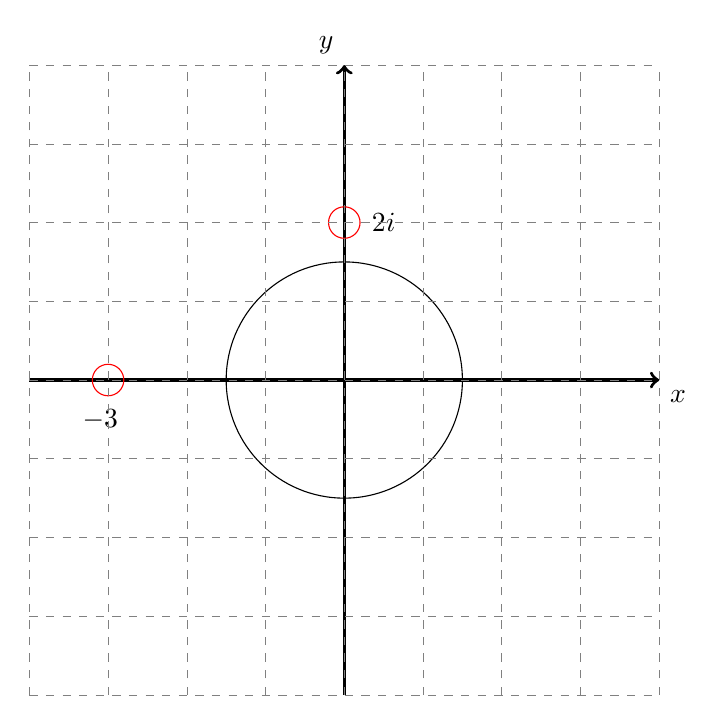
\begin{tikzpicture}
\draw[very thick,->] (-4,0) -- (4,0) node[anchor=north west] {$x$};
\draw[very thick,->] (0,-4) -- (0,4) node[anchor=south east] {$y$};
\draw (0,0) circle (1.5cm);

\draw[red] (0,2) circle (2mm) ;
\draw[red] (-3,0) circle (2mm) ;


\node at (0.5,2) {$2i$};
\node at (-3.1,-0.5) {$-3$};


\draw[step=1cm,gray,dashed,very thin] (-4,-4) grid (4,4);
\end{tikzpicture}

Η $f$ είναι αναλυτική στο εσωτερικό και πάνω  στην απλή κλειστή τμηματικά λεία καμπύλη $C_{R}$. Άρα $Ι=0$.

\begin{itemize}
\item Όταν έχουμε $2<R<3$ :
\end{itemize}

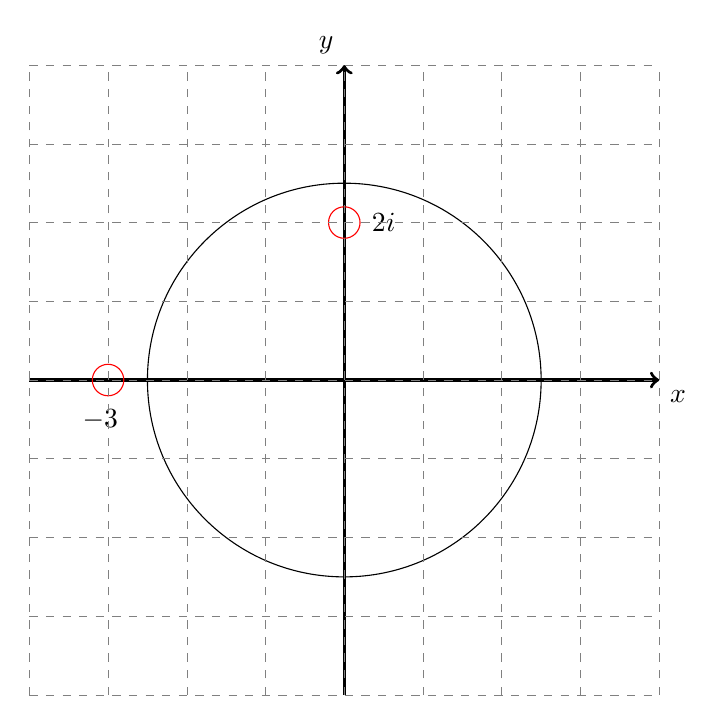
\begin{tikzpicture}
\draw[very thick,->] (-4,0) -- (4,0) node[anchor=north west] {$x$};
\draw[very thick,->] (0,-4) -- (0,4) node[anchor=south east] {$y$};
\draw (0,0) circle (2.5cm);

\draw[red] (0,2) circle (2mm) ;
\draw[red] (-3,0) circle (2mm) ;


\node at (0.5,2) {$2i$};
\node at (-3.1,-0.5) {$-3$};


\draw[step=1cm,gray,dashed,very thin] (-4,-4) grid (4,4);
\end{tikzpicture}
\newline
Η $f$ είναι αναλυτική στο εσωτερικό και πάνω  στην απλή κλειστή τμηματικά λεία καμπύλη $C_R$ με εξαίρεση το σημείο $z=-2i$ το οποίο βρίσκεται στο εσωτερικό της. Άρα 
$$Ι=2 \pi i Res(f,2i)= \frac{(24+10i)\pi}{169} $$.
\\
Όπου :
$$ Res(f,2i)= \lim_{z\to 2i} \frac{(z-2i)}{(z-2i)(z+3)^2}= \lim_{z\to 2i} \frac{1}{(z+3)^2} = \frac{1}{(3+2i)^2}= $$
$$=\frac{1}{5+12i}=\frac{5-12i}{25+144}=\frac{5-12i}{169}$$

\begin{itemize}
\item Όταν έχουμε $R>3$ :
\end{itemize}

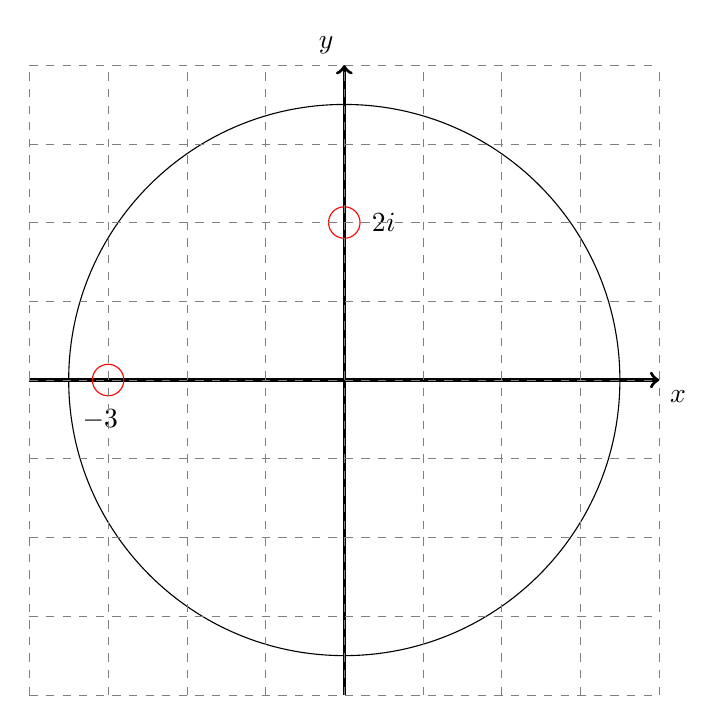
\begin{tikzpicture}
\draw[very thick,->] (-4,0) -- (4,0) node[anchor=north west] {$x$};
\draw[very thick,->] (0,-4) -- (0,4) node[anchor=south east] {$y$};
\draw (0,0) circle (3.5cm);

\draw[red] (0,2) circle (2mm) ;
\draw[red] (-3,0) circle (2mm) ;


\node at (0.5,2) {$2i$};
\node at (-3.1,-0.5) {$-3$};


\draw[step=1cm,gray,dashed,very thin] (-4,-4) grid (4,4);
\end{tikzpicture}
\newline
Η $f$ είναι αναλυτική στο εσωτερικό και πάνω  στην απλή κλειστή τμηματικά λεία καμπύλη $C_{R}$ με εξαίρεση τα σημεία $z=2i$ και $ z=-3$ τα οποία βρίσκονται στο εσωτερικό της. Άρα
$$ Ι= 2 \pi i \left( Res(f,2i)+ Res(f,-3) \right)= 0 $$
\\
Όπου :
$$ Res(f,2i)= \lim_{z\to 2i} \frac{(z-2i)}{(z-2i)(z+3)^2}= \lim_{z\to 2i} \frac{1}{(z+3)^2} = \frac{1}{(3+2i)^2}= $$
$$=\frac{1}{5+12i}=\frac{5-12i}{25+144}=\frac{5-12i}{169}$$

$$ Res(f,-3)= \lim_{z\to -3} \left[ \frac{(z+3)^2}{(z-2i)(z+3)^2} \right]'= \lim_{z\to -3} \left( \frac{1}{z-2i} \right)' = $$
$$= \lim_{z\to -3} - \frac{1}{(z-2i)^2} =-\frac{1}{(3+2i)^2}=-\frac{1}{5+12i}=-\frac{5-12i}{25+144}=-\frac{5-12i}{169}$$
\\

 \subsection{Άσκηση 5}

Θεωρούμε την $ g(z)=\frac{f(z)}{z^2} ,z \in D$ η οποία είναι αναλυτική στο $D$ και συνεχής στο σύνορο $\partial D$ αφού είναι και η $ f $.
Τότε 
$$ |g(z)|=\frac{|f(z)|}{|z|^2} \quad (1) $$
\\
Για $ z:|z|=1, \quad (1)\Rightarrow |g(z)|=|f(z)|\leq 1 $\\
Για $ z:|z|=3, \quad (1)\Rightarrow |g(z)|=\frac{|f(z)|}{9}\leq \frac{9}{9}\Rightarrow |g(z)|\leq 1 $
\\ \\
Από το Θεώρημα Μεγίστου, αφού η $g$ είναι αναλυτική στο $D$ και συνεχής στο σύνορο $\partial D$, η $|g(z)|$ παίρνει μέγιστο πάνω στο $\partial D$, δηλαδή $|g(z)|\leq1,\forall z \in D \Rightarrow |f(z)|\leq |z|^2,\forall z \in D $
 \subsection{Άσκηση 6}

$$ f(z)=\frac{iz+1}{z^3-z^2+z-1} $$

Έχουμε:
$$ z^3-z^2+z-1=z(z^2+1)-(z^2+1)=(z-1)(z+i)(z-i) $$

Άρα 
$$ f(z)=\frac{i(z-i)}{(z-1)(z+i)(z-i)} \Rightarrow f(z)=\frac{i}{(z-1)(z+i)} , \quad z \in \mathbb{C}-\{-i,i,1\} $$

Έστω $A,B\in\mathbb{C}$ τέτοια ώστε:

$$ \frac{A}{z-1}+\frac{B}{z-i}= \frac{i}{(z-1)(z+i)} \Rightarrow A(z-i)+B(z-1)=i \Rightarrow$$


\[
\spalignsys{A+B=0;-iA-B=i} \Rightarrow \spalignsys{A=-B;-iA+A=i}\Rightarrow \spalignsys{-A=B;A=\frac{i}{1-i} }\Rightarrow \spalignsys{ B=\frac{1-i}{2};A=\frac{-1+i}{2}}
\]

$$ f(z)= \frac{-1+i}{2} \left( \frac{1}{z-1} \right)  + \frac{1-i}{2} \left( \frac{1}{z+i} \right)\Rightarrow f(z)= \frac{1-i}{2} \left( \frac{1}{1-z} \right)  + \frac{1-i}{2i} \left( \frac{1}{1-iz} \right)\Rightarrow  $$

$$ \Rightarrow f(z)= \left(\frac{1-i}{2}\right) \sum_{n=0}^{\infty}{z^n}  + \left(\frac{1-i}{2i} \right) \sum_{n=0}^{\infty}{(iz)^n} ,|z|<1$$

 \subsection{Άσκηση 7}

$$I= \int_{-\infty}^{+\infty} \frac{dx}{x^3+8}$$
\\ Λύνουμε

$$ z^3+8=0 \Rightarrow z^3=-8 \Rightarrow
z=\sqrt[3]{|-8|}e^{i \left(\frac{\pi + 2\kappa \pi}{3} \right) } , \kappa=\{0,1,2\}\Rightarrow $$
\\
$ z=2e^{i\frac{\pi}{3}}= 1+i\sqrt{3} \quad $ή$ \quad z=-2 \quad $ή$ \quad z=2e^{i\frac{5\pi}{3}}=1-i\sqrt{3} $
\\
\\
Θέτουμε $ f(z)=\frac{1}{z^3+8},z\in\mathbb{C}-\{-2, 1+i\sqrt{3},1-i\sqrt{3}\} $
\\ \\
Άρα έχουμε τρείς πόλους πρώτης τάξης, έναν στο άνω, έναν στο κάτω ημιεπίπεδο και έναν πάνω στον πραγματικό άξονα.

$$ \lim_{z \to \infty } zf(z)=\lim_{z \to \infty } \frac{z}{z^3+8}=
\lim_{z \to \infty } \frac{z}{z^3\left(1+\frac{8}{z^3}\right)}=
\lim_{z \to \infty } \frac{1}{z^2\left(1+\frac{8}{z^3}\right)} =0$$

Επομένως $$ Ι= 2 \pi i Res(f,1+i\sqrt{3})+ \pi i Res(f,-2)\quad (1) $$

$$  Res(f,-2)=\lim_{z\to -2}\frac{z+2}{(z+2)(z-(1+i\sqrt{3}))(z-(1-i\sqrt{3}))}=$$
$$=\frac{1}{(-3-i\sqrt{3})(-3+i\sqrt{3})}=\frac{1}{9+3}=\frac{1}{12}$$

$$ Res(f,1+i\sqrt{3})=\lim_{z\to (1+i\sqrt{3})} \left[ \frac{z-(1+i\sqrt{3})}{(z+2)(z-(1+i\sqrt{3}))(z-(1-i\sqrt{3}))} \right]= $$

$$=\frac{1}{2i\sqrt{3}(3+i\sqrt{3})}= \frac{3-i\sqrt{3}}{2i\sqrt{3}(9+3)} = \frac{\sqrt{3}-i}{12(2i)}  $$
\\
Άρα η $(1)$ γίνεται:
\\
$$ Ι=2\pi i \left[ \frac{\sqrt{3}-i}{12(2i)} \right] + \pi i \left( \frac{1}{12} \right) =
\frac{\pi \sqrt{3}-i\pi+i\pi}{12} = \frac{\pi \sqrt{3}}{12}$$
\\
Άρα $$ \int_{-\infty}^{+\infty} \frac{dx}{x^3+8}= \frac{\pi \sqrt{3}}{12} $$
\newpage



\newpage \part{Εφαρμοσμένα Μαθηματικά Φεβρουάριος 2015}
\author{}


  

\maketitle
\newpage
 

 \section{Θέματα Ατρέα}
 \subsection{Άσκηση 1}
$$z^4=(-i)^{2i}=e^{2ilog(-i)}=e^{2i[ln(|-i|)+i(-\frac{\pi}{2}+2 \kappa \pi)]}=e^{\pi-4\kappa \pi}=e^{\pi(1-4\kappa)}\Rightarrow
$$
$$\Rightarrow
z=\sqrt[4]{|e^{\pi(1-4\kappa)}|}e^{\frac{2\lambda\pi i}{4}}
=\sqrt[4]{e^{\pi(1-4\kappa)}}e^{\frac{\lambda\pi i}{2}}
$$με $\kappa\in \mathbb{Z},\lambda={0,1,2,3}$ 
\\
Άρα

\[
z= 
\spalignsys 
{\sqrt[4]{e^{\pi(1-4\kappa)}};
i\sqrt[4]{e^{\pi(1-4\kappa)}};
-\sqrt[4]{e^{\pi(1-4\kappa)}};
-i\sqrt[4]{e^{\pi(1-4\kappa)}}
 }
 \quad,\kappa \in \mathbb{Z}
\]
\newpage
 \subsection{Άσκηση 2}
α) $
\Omega = \{z \in \mathbb{C}:|z|<2 , \pi/3  < Arg(z) <
 5\pi /4 \}
$
\\
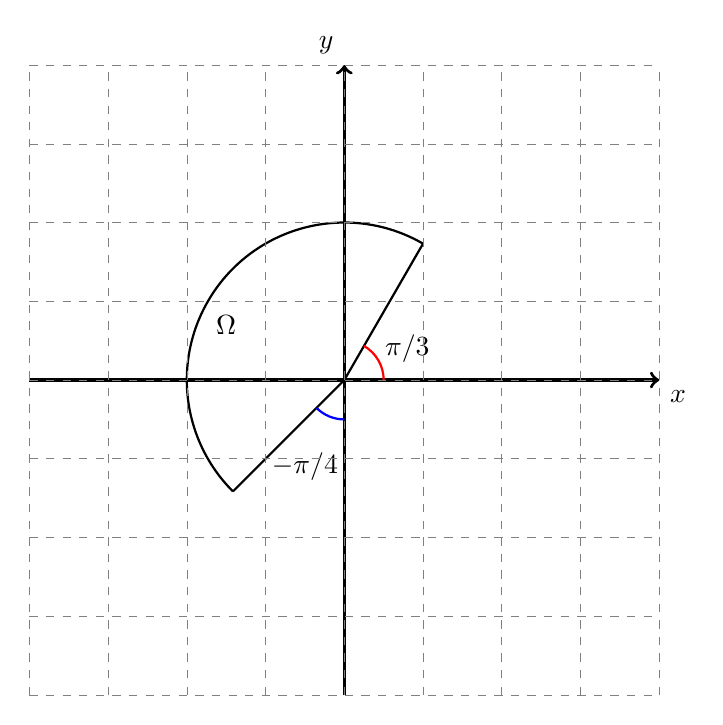
\begin{tikzpicture}
\draw[very thick,->] (-4,0) -- (4,0) node[anchor=north west] {$x$};
\draw[very thick,->] (0,-4) -- (0,4) node[anchor=south east] {$y$};
\draw[thick] (0,0) -- ++(60:2cm)
      (0,0) -- ++(225:2cm);
\draw[thick,black] ([shift=(60:2cm)]0,0) arc (60:225:2cm);
\draw[thick,red] ([shift=(0:0.5cm)]0,0) arc (0:60:0.5cm);
\draw[thick,blue] ([shift=(225:0.5cm)]0,0) arc (225:270:0.5cm);
\node at (0.8,0.4) {$\pi/3$};
\node at (-0.5,-1.1) {$-\pi/4$};
\node at (-1.5,0.7) {$\Omega$};
\draw[step=1cm,gray,dashed,very thin] (-4,-4) grid (4,4);

\end{tikzpicture}
\newline

β)
\[
\spalignsys{f(z)=2\sqrt{z}=2z^{1/2};z=|z|e^{iArg(z)}}
\]
$$
f(z)=(|z|e^{iArg(z)})^{1/2}=2|z|^{1/2}e^{i\frac{Arg(z)}{2}}
$$

\[
f(z)=2(|z|e^{iArg(z)})^{1/2}=
\underbrace{2|z|^{1/2}}_{\text{$|f(z)|$}}
e^{i
\overbrace{\frac{Arg(z)}{2}}^{\text{$Arg(f(z))$}}
}
\]
$\bullet \quad
Arg(f(z))=\frac{Arg(z)}{2}\Rightarrow \frac{\pi}{6}
\leqslant Arg(f(z)) \leqslant \frac{5\pi}{6}
$
\newline
$\bullet \quad
|f(z)|=2|z|^{1/2} ,|f(z)|\leqslant 2\sqrt{2}
$
\newline
\newline

Άρα $f(\Omega)=\{|f(z)|\leqslant2\sqrt{2} ,\quad \frac{\pi}{6}\leqslant Arg(f(z)) \leqslant \frac{5\pi}{8}\}$
\newpage

γ )
\\$ \gamma(t)=e^{it} ,\quad t\in(-\pi,\pi] $ \\ $\gamma'(t)=ie^{it} $ 

$$\oint_{|z|=1} f(z)  \,dz = \int_{-\pi}^{\pi} 2e^{it/2}ie^{it}dt= $$
$$
=\int_{-\pi}^{\pi} 2ie^{i\frac{3t}{2}} dt =
\left[ \frac{2ie^{i\frac{3t}{2}}}{\frac{3i}{2}}
\right]_{-\pi}^{\pi}=\frac{3i}{4i}(e^{i\frac{3\pi}{2}}-e^{-i\frac{3\pi}{2}})=\frac{8i}{3}sin\left(\frac{3\pi}{2}\right)=-\frac{8i}{3}
$$
\newline 
\newline 
 \subsection{Άσκηση 3}
Η $f(z)=f(x+yi)=u(x,y)+iv(x,y)$ είναι αναλυτική στο $Ε$. \\
\\
Από τις εξισώσεις $Cauchy-Riemann$ έχουμε
\\
\[
\spalignsys {u_x=v_y;u_y=-v_x}
\]
\\Άρα:
\[
au+bv=c 
\Rightarrow
\spalignsys{au_x+bv_x=0;au_y+bv_y=0}
\Rightarrow
\]

\[
\Rightarrow
\begin{bmatrix}
    u_x & v_x \\
    u_y & v_y 
\end{bmatrix}
\begin{bmatrix}
	a \\
	b
\end{bmatrix}
=
\begin{bmatrix}
0\\
0
\end{bmatrix}
\Leftrightarrow
\begin{bmatrix}
    u_x & -u_y \\
    u_y & u_x 
\end{bmatrix}
\begin{bmatrix}
	a \\
	b
\end{bmatrix}
=
\begin{bmatrix}
0\\
0
\end{bmatrix}
\]
Έχουμε ότι $ a,b \in \mathbb{C} $ με $ |a|^2+|b|^2\neq0 \Rightarrow a ,b \neq 0$. Eπομένως για το παραπάνω σύστημα έχουμε ότι \[ \begin{vmatrix}
u_x & -u_y \\
    u_y & u_x
\end{vmatrix}=u_x^2+u_y^2 \quad (1)
\]
Έστω ότι η $(1)$ είναι 0. Τότε το παραπάνω σύστημα θα είχε μοναδική λύση, τη μηδενική (αφού το σύστημα είναι ομογενές) το οποίο είναι άτοπο καθώς $a ,b \neq 0$.
\\
\\
Έτσι από την $(1)$ έχουμε ότι  $u_x^2+u_y^2=0 \Rightarrow u_x=u_y=v_y=v_x=0$ λόγω των εξισώσεων $Cauchy-Riemann$  και $f_x=u_x+iv_x=0\Rightarrow \quad f(z)=c,c\in\mathbb{C}$ στο $E$
\newpage
 \subsection{Άσκηση 4}
$$Ι=\oint_{C} \frac{e^z-cos(z)}{(z-i)(z-2)^{4}sin^2(z)}  \,dz$$

Θεωρούμε την  $f(z)=\frac{e^z-cos(z)}{(z-i)(z-2)^{4}sin^2(z)},z\in\mathbb{C}-\{0,2,i\}$.


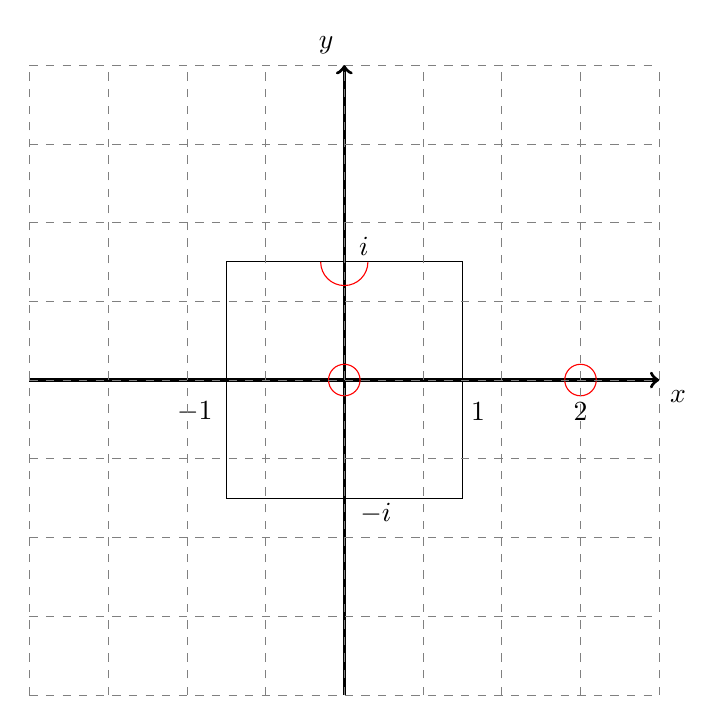
\begin{tikzpicture}
\draw[very thick,->] (-4,0) -- (4,0) node[anchor=north west] {$x$};
\draw[very thick,->] (0,-4) -- (0,4) node[anchor=south east] {$y$};

\draw (-1.5,1.5) -- (-1.5,-1.5) -- (1.5,-1.5) -- (1.5,1.5)--(-1.5,1.5);
 
\draw[red] (0,0) circle (2mm) ;
\draw[red] (-0.3,1.5) arc (180:360:3mm); 
\draw[red] (3,0) circle (2mm) ;


\node at (3,-0.4) {$2$};
\node at (-1.9,-0.4) {$-1$};
\node at (1.7,-0.4) {$1$};
\node at (0.4,-1.7) {$-i$};
\node at (0.25,1.7) {$i$};
\draw[step=1cm,gray,dashed,very thin] (-4,-4) grid (4,4);
\end{tikzpicture}
\newline
Το $z_1=0$ και το $z_2=i$ είναι απλοί πόλοι, ενώ το $z_3=2 \notin C$ (οπότε δεν μας αφορά). Άρα:

$$I=2\pi i Res(f,0) + \pi i Res(f,i)=-\frac{\pi}{8}
+\frac{\pi i (e^i-cos(i))}{(2-i)^4sin^2(i)}
$$ 
Όπου
$$
Res(f,i)=\lim_{z \rightarrow i}
\frac{\cancel{(z-i)}(e^z-cos(z))}{\cancel{(z-i)}(z-2)^{4}sin^2(z)}
=
\frac{(e^i-cos(i))}{(i-2)^{4}sin^2(i)}
$$
$$Res(f,0)=\lim_{z \rightarrow 0}\frac{z(e^z-cos(z))}{(z-i)(z-2)^{4}sin^2(z)}=\frac{i}{16}
$$
Αφού 
$$\lim_{z \rightarrow 0}\frac{e^z-cos(z)}{sin(z)} 
\overset{\mathrm{De L'Hospital}}{=\joinrel=\joinrel=\joinrel=\joinrel=\joinrel=\joinrel=}
\lim_{z \rightarrow 0}\frac{e^z-sin(z)}{cos(z)} 
=1
$$

$$
\lim_{z\rightarrow 0} \frac{z}{sin(z)}
\overset{\mathrm{DLH}}{=\joinrel=\joinrel=}
\lim_{z\rightarrow 0} \frac{1}{cos(z)}=1
$$

$$
\lim_{z \rightarrow 0} \frac{1}{(z-i)(z-2)^{4}}=
\frac{1}{(-i)16}=\frac{i}{16}
$$
\newpage
 \subsection{Άσκηση 5}
$$f(z)=(2z^2-z)e^{\frac{2}{z-2}}
$$
Γενικά έχουμε ότι : $$\bullet\quad(2z^2-z)=2(z-2)^2+7(z-2)+6$$  
$$\bullet\quad e^{\frac{2}{z-2}}=\sum_{n=0}^\infty \frac{1}{n!}\left[\frac{2}{z-2}\right]^n $$ 
Άρα: 
$$
f(z)=\left(\sum_{n=0}^\infty \frac{1}{n!}\left[\frac{2}{z-2}\right]^n
\right)
\left(
2(z-2)^2+7(z-2)+6
\right)=
$$
$$
=\frac{1}{0!}\left[
2(z-2)^2+7(z-2)+6
\right]
+\frac{1}{1!}\frac{2}{z-2}\left[
2(z-2)^2+7(z-2)+6
\right]+$$
$$
+\frac{1}{2!}\frac{2^2}{(z-2)^2}\left[
2(z-2)^2+7(z-2)+6
\right]
+ \frac{1}{3!}\frac{2^3}{(z-3)^3}\left[
2(z-2)^2+7(z-2)+6
\right]+\ldots
$$
\\
Συνεπώς:
$$
Res(f,2)=\frac{2\cdot6}{1!}+
\frac{2^2\cdot7}{2!}+\frac{2^3\cdot2}{3!}
=\frac{86}{3}
$$
\newpage
 \subsection{Άσκηση 6}
Θέλουμε να βρούμε τη σειρά $Laurent$ με κέντρο το $z_0=i \quad \forall z : 2<|z-z_0|<3 $ 
$$
f(z)=\frac{2iz+3-i}{iz^2+z+6i}=
\frac{2z-3i-1}{z^2-iz+6}=\frac{2z-(1+3i)}{(z+2i)(z-3i)}=\frac{z-i}{5(z+2i)}+
\frac{3+i}{5(z-3i)}\Rightarrow
$$
$$\Rightarrow f(z)=
\frac{(7-i)}{15i}\sum_{n=0}^{\infty} \left(\frac{z-i}{3i} \right)^n 
+
\frac{(3+i)}{5(z-i)}\sum_{n=0}^{\infty} \left(\frac{2i}{z-i} \right)^n \Rightarrow$$
$$
\Rightarrow 
f(z)=
\frac{(1-7i)}{15}\sum_{n=0}^{\infty} \left(\frac{z-i}{3i} \right)^n 
+
\frac{(3+i)}{5}\sum_{n=0}^{\infty} \frac{(2i)^n}{(z-i)^{n+1}} \quad, \quad 2<|z-i|<3
$$

 \subsection{Άσκηση 7}
$$
A,B,C > 0  \qquad |f(z)|\leqslant A|z|^2+B|z|+C
$$
Αν $f$ πολυώνυμο το πολύ 2ου βαθμού 
$f(z)=az^2+bz+c,\quad a,b,c\in \mathbb{C}$ τότε 
$f'(z)=2az+b,\quad f''(z)=2a ,\quad f^{(3)}(z)=0
$
\\\\Έχουμε ότι : $|f^{(n)}(z)|\leqslant \frac{n!M_r}{R^n}$ και 
\[
M_r=max\{|f(z)|:
\underbrace{|z-z_o|=R}_{\text{$z=z_o+Re^{i\theta}$}}
\}
\]
\\
Αρκεί να δείξουμε ότι $f^{(3)}(z)=0,\forall z \in \mathbb{C}$
$$
|f(z)|\leqslant A|z|^2+B|z|+C=A|z_o+Re^{i\theta}|^2+B|z_o+Re^{i\theta}|+C
\leqslant$$$$
\leqslant
A(|z_o|+R|e^{i\theta}|)^2+B|z_o|+BR|e^{i\theta}|+C=
A|z_o|^2+2AR|z_o|+AR^2+B|z_o|+BR+C
\Rightarrow$$
$$\Rightarrow
|f^{(3)}(z)|\leqslant\frac{3!(
A|z_o|^2+2AR|z_o|+AR^2+B|z_o|+BR+C)}{R^3}
\overset{\mathrm{R\rightarrow +\infty}}{\Rightarrow}
$$
$$
\Rightarrow
|f^{(3)}(z)|\leqslant0 \Rightarrow f^{(3)}(z)
=0
$$
\newpage
 \subsection{Άσκηση 8}
$$
I=\int_{-\infty}^{+\infty}\frac{dx}{(x^2+a^2)^2(x-1)},\quad a>0
$$ \\
Θεωρούμε την $f(z)=\frac{1}{(z^2+a^2)^2(z-1)},z\in \mathbb{C}-\{-a i,a i,1 \}
$
\\  \\
Η $f$ έχει τρείς πόλους.
\begin{itemize}
\item $z_0=1$ ,απλός πόλος πάνω στον πραγματικό άξονα
\item $z_1=ai$ ,διπλός πόλος στο άνω ημιεπίπεδο ( αφού $a>0$ )
\item $z_2=-ai$ ,διπλός πόλος στο κάτω ημιεπίπεδο ( αφού $a>0$ )
\\
\end{itemize}

Έχουμε: 
$$\lim_{z \rightarrow \infty} zf(z)=\lim_{z \rightarrow \infty} \frac{z}{(z^2+a^2)^2(z-1)}=\lim_{z \rightarrow \infty} \frac{z}{z(z^2+a^2)^2(1-\frac{1}{z})}=\lim_{z \rightarrow \infty} \frac{1}{(z^2+a^2)^2(1-\frac{1}{z})}=0$$
\\ \\
Άρα $I=2\pi i Res(f,ai)+\pi i Res(f,1)= -\frac{(3a^2+1)\pi}{2a^3(a^2+1)^2}$
\\
$$ \bullet\quad Res(f,1)=\lim_{z \rightarrow 1}\left[\frac{\cancel{(z-1)}}{\cancel{(z-1)}(z^2+a^2)^2}\right]=\frac{1}{(1+a^2)^2}
\quad(1)$$

$$
\bullet\quad Res(f,ai)=\lim_{z \rightarrow ai}\left[\frac{\cancel{(z-ai)^2}}{\cancel{(z-ai)^2}(z+ai)^2(z-1)}\right]'=
$$
$$=\lim_{z \rightarrow ai}-\frac{2(z+ai)(z-1)+(z+ai)^2}{(z+ai)^4(z-1)^2}=
\frac{4ai(ai-1)+(2ai)^2}{-(2ai)^4(ai-1)^2}=
$$
$$
=-\frac{2}{(2ai)^3(ai-1)}-\frac{1}{(2ai)^2(ai-1)^2}=
\frac{2(-ai-1)}{8a^3i(a^2+1)}+\frac{(-ai-1)^2}{4a^2(a^2+1)^2}\quad(2)$$

$$
(1),(2) \Rightarrow 
I =  \frac{\pi i}{(1+a^2)^2}+\frac{\pi(-ai-1)}{2a^3(a^2+1)}+\frac{\pi i(-ai-1)^2}{2a^2(a^2+1)^2}=
$$
$$
\Rightarrow I=
\frac{\pi i(2a^3)+\pi(-1-ai)(a^2+1)+\pi i(1+ai)^2a}{2a^3(1+a^2)^2}
$$
$$
\Rightarrow I=
\frac{\pi(-a^2-1-a^3i-ai)+\pi(ia-2a^2-a^3i)+\pi i(2a^3)}
{2a^3(1+a^2)^2}=-\frac{(3a^2+1)\pi}{2a^3(a^2+1)^2}
$$
\\
Άρα 
$$\int_{-\infty}^{+\infty}\frac{dx}{(x^2+a^2)^2(x-1)} =-\frac{(3a^2+1)\pi}{2a^3(a^2+1)^2} \quad,a>0 $$
 

\newpage \part{Εφαρμοσμένα Μαθηματικά Σεπτέμβριος 2014}
\author{}


  

\maketitle
\newpage
 

 \section{Θέματα Ατρέα}
 \subsection{Άσκηση 1}

Θέτουμε $\quad c=a+bi ,\quad d=m+ni , \quad a,b,m,n \in \mathbb{R} \quad $ και \\
$ \quad a^2+b^2\neq 0 , \quad m^2+n^2\neq 0 $

$$ \frac{c}{d}=\frac{a+bi}{m+ni}=\frac{(a+bi)(m-ni)}{m^2+n^2}=\frac{am+bn}{m^2+n^2} + i \frac{bm-an}{m^2+n^2} \quad (1)  $$

$$ \frac{d}{c}=\frac{m+ni}{a+bi}=\frac{(m+ni)(a-bi)}{a^2+b^2}=\frac{am+bn}{a^2+b^2} + i \frac{an-bm}{a^2+b^2} \quad (2) $$
\\
Από τις $(1),(2)$ έχουμε:

$$ Im\left(\frac{c}{d}\right) < 0 \Leftrightarrow  
\frac{bm-an}{m^2+n^2}<0 \Leftrightarrow bm-an<0 \Leftrightarrow
an-bm>0
\Leftrightarrow
\frac{an-bm}{a^2+b^2}>0 
\Leftrightarrow 
Im\left(\frac{d}{c}\right) > 0
$$

\newpage
 \subsection{Άσκηση 2}

$$ \sin(iz)+ i\sinh(z)=i \quad (1)$$
Θέτουμε $z=x+yi, \quad x,y\in \mathbb{R}$ κι έχουμε:\\

$$ \sin(iz)=\frac{e^{i [i(x+yi)]}-e^{-i[i(x+yi)]}}{2i} = -i \frac{e^{-(x+yi)}-e^{x+yi}}{2}= i\sinh(z) $$
Άρα η (1) γίνεται:

$$
i\sinh(z)+i\sinh(z)=i \Rightarrow \sinh(z)=\frac{1}{2}\Rightarrow 
\frac{e^{x+yi}-e^{-(x+yi)}}{2}=\frac{1}{2} \Rightarrow $$

$$
\Rightarrow \frac{e^x}{2}(\cos(y)+i\sin(y))-\frac{e^{-x}}{2}(\cos(y)-i\sin(y))=\frac{1}{2} \Rightarrow$$
$$
\cos(y)\left[ \frac{e^x-e^{-x}}{2} \right]+i\sin(y)\left[ \frac{e^x+e^{-x}}{2} \right]=\frac{1}{2}
\Rightarrow
$$ 

$$ \Rightarrow \cos(y)\sinh(x)+i\sin(y)\cosh(x)=\frac{1}{2} \Rightarrow $$

\[
\Rightarrow
\spalignsys{ \cos(y)\sinh(x)=\frac{1}{2} ; ; \sin(y)\cosh(x)=0}
\Rightarrow
\spalignsys{ \cos(y)\sinh(x)=\frac{1}{2} ; ;  \sin(y)=0}
\overset{(\ast)}{\Longrightarrow}
\spalignsys{\sinh(x)=\pm\frac{1}{2} ; ;  y = \kappa \pi {,} \quad  \kappa \in \mathbb{Z} }
\] 

$(\ast) \quad$  
Αν $\sin(y)=0$, τότε $ \cos(y)= \pm 1 $ ( λόγω της γνωστής τριγωνομετρικής ταυτότητας $\sin^2(\alpha)+\cos^2(\alpha)=1, \quad \forall \alpha \in \mathbb{R} \quad)$\\

$$\bullet \quad \sinh(x)= \frac{1}{2} \Rightarrow \frac{e^x-e^{-x}}{2}=  \frac{1}{2} \Rightarrow
e^{2x}-1=  e^x \Rightarrow e^{2x}-e^x -1=0 \quad (2) $$

Θέτουμε $ w=e^x, \quad w>0 $ και $(2)$ γίνεται:

$$ w^2-w-1=0 $$
 $$ \Delta=1+4=5>0, \qquad  w=\frac{1\pm \sqrt{5}}{2}$$
 Όμως $w>0$, άρα $ w=\frac{1 + \sqrt{5}}{2}$
 
 $$ e^x=\frac{1 + \sqrt{5}}{2} \Rightarrow x= \ln\left( \frac{1 + \sqrt{5}}{2} \right) $$
 
 $$\bullet \quad  \sinh(x)= -\frac{1}{2} \Rightarrow \frac{e^x-e^{-x}}{2}=  -\frac{1}{2} \Rightarrow
e^{2x}-1=  -e^x \Rightarrow e^{2x}+e^x -1=0 \quad (3) $$

Θέτουμε $ u=e^x, \quad w>0 $ και $(3)$ γίνεται:

$$ u^2+u-u=0 $$
 $$ \Delta=1+4=5>0, \qquad  u=\frac{-1\pm \sqrt{5}}{2}$$
 Όμως $u>0$, άρα $ u=\frac{-1 + \sqrt{5}}{2}$
 
 $$ e^x=\frac{-1 + \sqrt{5}}{2} \Rightarrow x= \ln\left( \frac{-1 + \sqrt{5}}{2} \right) $$
 
Άρα

$$ z_1= \ln\left( \frac{1 + \sqrt{5}}{2} \right) +i \kappa \pi \quad , \quad  z_2=\ln\left( \frac{-1 + \sqrt{5}}{2} \right) +i \lambda \pi , \quad \kappa,\lambda \in \mathbb{Z} $$ 
 

 
 \newpage
 \subsection{Άσκηση 3}
(a)
$$ f(z)=w=\frac{iz-i}{2z-1+i} \Leftrightarrow 2zw-(1-i)w=iz-i \Leftrightarrow 2zw-iz=(1-i)w-i \Leftrightarrow $$
$$ \Leftrightarrow z(2w-i)= (1-i)w-i \Leftrightarrow 
 z=\frac{(1-i)w-i}{2w-i}=f^{-1}(w)$$
(b)
$$ \lim_{z \to \infty} f(z)= \lim_{z \to \infty}\frac{iz-i}{2z-1+i}=\lim_{z \to \infty}\frac{z\left(i-\frac{i}{z}\right)}{z\left(2-\frac{1-i}{z}\right)}=\lim_{z \to \infty}\frac{i-\frac{i}{z}}{2-\frac{1-i}{z}}=\frac{i}{2}   $$
(γ)
Θέτουμε $w=x+yi, x,y \in \mathbb{R}$ και $f^{-1}(w)=u+iv$
$$Im(w)=1 \Rightarrow y=1 $$
Άρα $w=x+i$
$$ f^{-1}(w)=\frac{(1-i)w-i}{2w-i} \Rightarrow u+iv=\frac{(1-i)(x+i)-i}{2(x+i)-i} \Rightarrow
u+iv=\frac{x-ix+1}{2x+i} \Rightarrow$$
$$ \Rightarrow u+iv=\frac{(x+1-ix)(2x-i)}{4x^2+1} \Rightarrow u+iv=\frac{(2x^2+x)-i(2x^2+x+1)}{4x^2+1} $$
\\ \\
$$ u=\frac{2x^2+x}{4x^2+1} \quad (1)  \qquad v=-\frac{2x^2+x+1}{4x^2+1} \quad (2)$$

$$ (1),(2)\Rightarrow u+v=-\frac{1}{4x^2+1} \Rightarrow 4x^2+1=-\frac{1}{u+v} \Rightarrow 4x^2=-\frac{u+v}{u+v}-\frac{1}{u+v} \Rightarrow $$
$$ \Rightarrow x^2=-\frac{1+u+v}{4(u+v)} \quad (3) $$

$$ (1)\Rightarrow u(4x^2+1)-2x^2=x \Rightarrow x^2=[u(4x^2+1)-2x^2]^2 \overset{(3)}{\Longrightarrow}$$

$$\Rightarrow -\frac{1+u+v}{4(u+v)} = \left[-\frac{u}{u+v}+\frac{1+u+v}{2(u+v)}\right]^2 
\Rightarrow -\frac{1+u+v}{4(u+v)} = \left[-\frac{2u}{2(u+v)}+\frac{1+u+v}{2(u+v)}\right]^2 \Rightarrow$$
$$ \Rightarrow -\frac{1+u+v}{4(u+v)} = \frac{(v-u+1)^2}{4(u+v)^2} \Rightarrow -(1+u+v)=\frac{v^2+u^2+1-2uv+2v-2u}{u+v} \Rightarrow $$
$$
\Rightarrow -(1+u+v)(u+v)=v^2+u^2+1-2uv+2v-2u \Rightarrow $$
$$\Rightarrow -u-v-u^2-uv-uv-v^2=v^2+u^2+1-2uv+2v-2u \Rightarrow $$
$$\Rightarrow 2v^2+2u^2+3v-u+1=0 \Rightarrow   u^2+v^2-\frac{1}{2}u+\frac{3}{2}v=-\frac{1}{2} \Rightarrow $$
$$\Rightarrow  u^2-2\left(\frac{1}{4}\right)u+\frac{1}{16}+v^2+2\left(\frac{3}{4}\right)v+\frac{9}{16}=-\frac{1}{2}+\frac{1}{16}+\frac{9}{16} \Rightarrow $$
$$\Rightarrow  \left( u-\frac{1}{4} \right)^2+\left( v+\frac{3}{4} \right)^2=\frac{1}{8} \Rightarrow $$
$$ \Rightarrow  \left( u-\frac{1}{4} \right)^2+\left( v+\frac{3}{4} \right)^2=\left(\frac{\sqrt{2}}{4}\right)^2 $$
Κύκλος με κέντρο το $Κ\left(\frac{1}{4},-\frac{3}{4}\right)$ και ακτίνα $r=\frac{\sqrt{2}}{4}$ 
\newpage
 \subsection{Άσκηση 4}

$$ u(x,y)=\sin(x)\sinh(y) $$
$$ u_x=\cos(x)\sinh(y) \qquad  u_{xx}=-\sin(x)\sinh(y)$$
$$ u_y=\sin(x)\cosh(y) \qquad  u_{yy}=\sin(x)\sinh(y) $$

$$ u_{xx}+u_{yy}=-\sin(x)\sinh(y)+\sin(x)\sinh(y)=0 $$

Άρα η $f$ είναι αρμονική.
\\ \\
Από τις εξισώσεις $Cauchy-Riemann$ έχουμε
\\
\[
\spalignsys {u_x=v_y; ;u_y=-v_x} \Rightarrow    
\spalignsys 
{v_y=\cos(x)\sinh(y); ; v_x=-\sin(x)\cosh(y)}
\Rightarrow
\]

\[
\Rightarrow
\spalignsys {v =\int \cos(x) \sinh(y)dy+h(x) ; ; v_x =-\sin(x)\cosh(y) } \Rightarrow    
\spalignsys 
{v=\cos(x)\cosh(y)+h(x); ;-\sin(x)\cosh(y)+h'(x)=-\sin(x)\cosh(y)}
\Rightarrow
\]

\[
\Rightarrow
\spalignsys {v=\cos(x)\cosh(y)+h(x) ; ;-\sin(x)\cosh(y)+h'(x)=-\sin(x)\cosh(y)}
\Rightarrow
\]

\[
\Rightarrow
\spalignsys {v=\cos(x)\cosh(y)+h(x); ; h'(x)=0 } \Rightarrow    
\spalignsys 
{v=\cos(x)\cosh(y)+c_1 ; ;  h(x)=c_1}
,\quad c_1 \in \mathbb{R}
\]
\\ \\
Άρα $ v(x,y) =\cos(x)\cosh(y)+c_1,\quad c_1 \in \mathbb{R} $
\\ \\
και
$$ f(z)=u(z,0)+iv(z,0)=i\cos(z)+i c_1 \Rightarrow$$
$$  \Rightarrow f(z)=i\cos(z)+c, \quad c\in \mathbb{C}  $$

\newpage
 \subsection{Άσκηση 5}

$$Ι=\oint_{C} \frac{e^z-z-1}{z^2(z-i)^2(z+1)} ,dz$$

Θεωρούμε την  $f(z)=\frac{e^z-z-1}{z^2(z-i)^2(z+1)},\quad z\in\mathbb{C}-\{-1,0,i\}$.


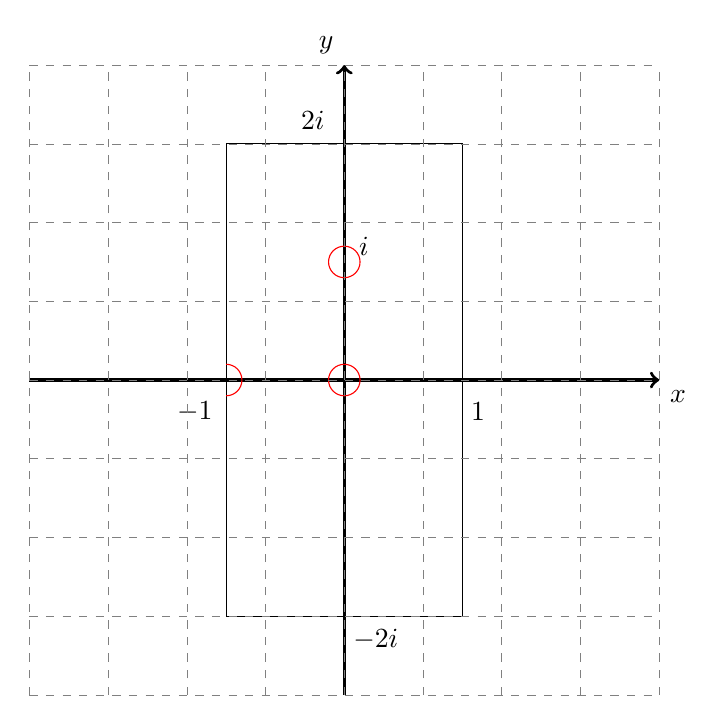
\begin{tikzpicture}
\draw[very thick,->] (-4,0) -- (4,0) node[anchor=north west] {$x$};
\draw[very thick,->] (0,-4) -- (0,4) node[anchor=south east] {$y$};

\draw (-1.5,3) -- (-1.5,-3) -- (1.5,-3) -- (1.5,3)--(-1.5,3);
 
\draw[red] (0,0) circle (2mm) ;
\draw[red] (-1.5,-0.2) arc (270:450:2mm); 
\draw[red] (0,1.5) circle (2mm) ;


\node at (-0.4,3.3) {$2i$};
\node at (-1.9,-0.4) {$-1$};
\node at (1.7,-0.4) {$1$};
\node at (0.4,-3.3) {$-2i$};
\node at (0.25,1.7) {$i$};
\draw[step=1cm,gray,dashed,very thin] (-4,-4) grid (4,4);
\end{tikzpicture}
\newline

Έχουμε μία απαλείψιμη ανωμαλία, την $z_0=0 \quad$ , έναν διπλό πόλο στο εσωτερικό της καμπύλης, τον $z_1=i \quad$ κι έναν απλό πόλο πάνω στο σύνορο, τον $z_2=-1, \quad$άρα:

$$I=2\pi i Res(f,i) + \pi i Res(f,-1)= 2\pi i \left[ \frac{e^i(3+2i)-4i}{8(2i)} \right]+ \pi i \left( \frac{1}{2ie} \right)= $$
$$= \frac{\pi [e^i(3+2i)-4i]}{8}+\frac{\pi}{2e}= \frac{\pi e [e^i(3+2i)-4i] +4\pi}{8e}= $$
$$=\frac{\pi[e^{1+i}(3+2i)+4(\pi-ie)]}{8e} $$


διότι:

$$ \bullet \quad \lim_{z\to 0} \frac{e^z-z-1}{z^2}= \frac{1}{2} \in \mathbb{C}-\{0\}$$
απαλείψιμη ανωμαλία \\ \\
Αφού 
$$\lim_{z \to 0}\frac{e^z-z-1}{z^2} 
\overset{\mathrm{De L'Hospital}}{=\joinrel=\joinrel=\joinrel=\joinrel=\joinrel=\joinrel=}
\lim_{z \to 0}\frac{e^z-1}{2z} 
=\overset{\mathrm{De L'Hospital}}{=\joinrel=\joinrel=\joinrel=\joinrel=\joinrel=\joinrel=}
\lim_{z \to 0}\frac{e^z}{2}=\frac{1}{2}
$$

$$ \bullet \quad Res(f,i)=\lim_{z \to i}
\left[\frac{\cancel{(z-i)^2}( e^z -z -1)}{\cancel{(z-i)^2}z^2(z+1)}\right]'=
$$ 

$$=\lim_{z \to i}
\left[\frac{( e^z -1)z^2(z+1)-(e^z-z-1)[2z(z+1)+z^2]}{[z^2(z+1)]^4}\right]= 
$$

$$=\frac{-( e^i -1)(1+i)-(e^i-i-1)[2i(1+i)-1]}{[-(1+i)]^4}=\frac{(1-e^i)(1+i)+(e^i-1-i)(3-2i)}{16}= 
$$

$$=\frac{1+i-e^i-ie^i+3e^i-3-3i-2ie^i+2i-2}{16}=\frac{2e^i-3ie^i-4}{16}=\frac{e^i(3+2i)-4i}{8(2i)}$$


$$ \bullet \quad Res(f,-1)=\lim_{z \to -1}
\left[\frac{\cancel{(z+1)}( e^z -z -1)}{\cancel{(z+1)}z^2(z-i)^2}\right]=\frac{e^{-1}}{(1+i)^2}=\frac{1}{2ie}
$$ 


\newpage
 \subsection{Άσκηση 6}

$$ f(z)= (z^2-2z)e^{\frac{1}{z+1}} , \quad z\in \mathbb{C}-\{-1\} $$

$$ \bullet \quad z^2-2z=z^2+2z+1-4z-4+3=(z+1)^2-4(z+1)+3 $$

$$ \bullet \quad e^{\frac{1}{z+1}}=\sum_{n=0}^{\infty} \frac{1}{n!}\frac{1}{(z+1)^n} $$

Άρα 
$$f(z)= [(z+1)^2-4(z+1)+3]\sum_{n=0}^{\infty} \frac{1}{n!(z+1)^n}= $$

$$=[(z+1)^2-4(z+1)+3]\left[1+\frac{1}{z+1}+\frac{1}{2!(z+1)^2}+\frac{1}{3!(z+1)^3}+...\right]=$$

$$=(z+1)^2-4(z+1)+3+(z+1)-4+\frac{3}{z+1}+\frac{1}{2!}-\frac{4}{2!(z+1)}+$$
$$\frac{3}{2!(z+1)^2}+ \frac{1}{3!(z+1)}-\frac{4}{3!(z+1)^2}+\frac{3}{3!(z+1)^3}+...$$

Άρα 
$$Res(f,-1)=3-\frac{4}{2!}+\frac{1}{3!}=\frac{7}{6}$$

\newpage
 \subsection{Άσκηση 7}
$Laurent$ γύρω από το $ z_0=4i, \quad 0<|z-4i|<9$
$$f(z)= \frac{z+i}{z^2+iz+20}= \frac{z+i}{(z-4i)(z+5i)},\quad z\in \mathbb{C}-\{-5i,4i\}$$

Έστω $A,B \in \mathbb{C}$ τέτοια ώστε:
$$ \frac{z+i}{(z-4i)(z+5i)}= \frac{A}{z-4i}+ \frac{B}{z+5i} \Rightarrow z+i=A(z+5i)+B(z-4i) \Rightarrow $$

$$ \Rightarrow z+i=(A+B)z+i(5A-4B) \Rightarrow $$

\[
\spalignsys {A+B=1; ;5A-4B=1}
\Rightarrow
\spalignsys {A+B=1; ;5(A+B)-9B=1}
\Rightarrow
\spalignsys {A=1-B; ;5-9B=1}
\Rightarrow
\spalignsys {A=1-B; ;B=\frac{4}{9}}
\Rightarrow
\spalignsys {A=\frac{5}{9}; ;B=\frac{4}{9}}
\]
Άρα
$$ f(z)=\frac{5}{9(z-4i)}+ \frac{4}{9(z+5i)}=\frac{5}{9}\frac{1}{(z-4i)}+ \frac{4}{9}\frac{1}{[(z-4i)+9i]}=\frac{5}{9}\frac{1}{(z-4i)}+ \frac{4}{81i}\frac{1}{\left[1+\frac{z-4i}{9i}\right]} \Rightarrow$$ 

$$
\Rightarrow f(z)=\frac{5}{9}\frac{1}{(z-4i)}- \frac{4i}{81}\sum_{n=0}^{\infty}(-1)^n\left[\frac{z-4i}{9i}\right]^n , \quad  0<|z-4i|<9 $$

\newpage
 \subsection{Άσκηση 8}

$$
|f(z)|\leqslant C,\quad\forall z \in \mathbb{C}
$$

Έχουμε ότι : $|f^{(n)}(z)|\leqslant \frac{n!M_r}{R^n}$ και 
\[
M_r=max\{|f(z)|:|z-z_o|=R\}
\]
\\
Αρκεί να δείξουμε ότι: $f'(z)=0,\quad \forall z \in \mathbb{C}$
$$
|f'(z)|\leqslant\frac{1!C}{R}
\overset{\mathrm{R\rightarrow +\infty}}{\Longrightarrow} $$
$$ \Rightarrow |f'(z)|\leqslant0 \Rightarrow f'(z)=0$$





\newpage
 \subsection{Άσκηση 9}


$$I= \int_{-\infty}^{+\infty} \frac{dx}{x^3-27}$$
\\ Λύνουμε

$$ z^3-27=0 \Rightarrow z^3=27 \Rightarrow
z=\sqrt[3]{|27|}e^{i \left(\frac{ 2\kappa \pi}{3} \right) } , \kappa=\{0,1,2\} $$
Δηλαδή:
\\ \\
$ z=3  \quad $ή$ \quad z=3e^{i\frac{2\pi}{3}}=\frac{-3+3\sqrt{3}i}{2}  \quad $ή$ \quad z=3e^{i\frac{4\pi}{3}}=-\frac{3+3\sqrt{3}i}{2}   $
\\
\\
Θέτουμε $ f(z)=\frac{1}{z^3-27},z\in\mathbb{C}-\left\{3, \frac{-3+3\sqrt{3}i}{2}  ,-\frac{3+3\sqrt{3}i}{2} \right\} $
\\ \\
Άρα έχουμε τρείς πόλους πρώτης τάξης, έναν στο άνω, έναν στο κάτω ημιεπίπεδο και έναν πάνω στον πραγματικό άξονα.

$$ \lim_{z \to \infty } zf(z)=\lim_{z \to \infty } \frac{z}{z^3-27}=
\lim_{z \to \infty } \frac{z}{z^3\left(1-\frac{27}{z^3}\right)}=
\lim_{z \to \infty } \frac{1}{z^2\left(1-\frac{27}{z^3}\right)} =0$$

Επομένως $$ Ι= 2 \pi i Res\left(f,\frac{-3+3\sqrt{3}i}{2} \right)+ \pi i Res(f,3)\quad (1) $$

$$  Res(f,3)=\lim_{z\to 3}\frac{z-3}{(z-3)\left(z-\frac{-3+3\sqrt{3}i}{2} \right)\left(z+\frac{3+3\sqrt{3}i}{2} \right)}=$$
$$= \frac{1}{\left(3+\frac{3-3\sqrt{3}i}{2} \right)\left(3+\frac{3+3\sqrt{3}i}{2} \right)}= \frac{1}{ \frac{1}{4} \left[ 9  ^2 + \left( 3\sqrt{3}\right) ^2 \right]}=\frac{1}{27}$$

$$ Res\left(f,\frac{-3+3\sqrt{3}i}{2}\right)=\lim_{z\to \left(\frac{-3+3\sqrt{3}i}{2}\right)} \left[ \frac{z-\left(\frac{-3+3\sqrt{3}i}{2}\right)}{(z-3)\left[z-\left(\frac{-3+3\sqrt{3}i}{2} \right) \right]\left[z-\left( -\frac{3+3\sqrt{3}i}{2} \right)\right]} \right]=  $$

$$=\frac{1}{ \left( \frac{-3+3\sqrt{3}i}{2} -3 \right) \left( \frac{-3+3\sqrt{3}i}{2}+ \frac{3+3\sqrt{3}i}{2} \right) }= \frac{1}{3\sqrt{3}i\left( \frac{-9+3\sqrt{3}i}{2} \right)} = -\frac{2\left(9+3\sqrt{3}i\right)}{3\sqrt{3}i\left(9^2+(3\sqrt{3})^2\right)}= $$

$$ = -\frac{6\left(3+\sqrt{3}i\right)}{12\sqrt{3}i \cdot27} = -\frac{3+\sqrt{3}i}{27\sqrt{3}(2i)}=-\frac{\sqrt{3}+i}{27(2i)}  $$
\\
Άρα η $(1)$ γίνεται:
\\
$$ Ι=2\pi i \left[ -\frac{\sqrt{3}+i}{27(2i)} \right] + \pi i \left( \frac{1}{27} \right) =
\frac{\pi (-\sqrt{3})-i\pi+i\pi}{27} = -\frac{\pi \sqrt{3}}{27}$$
\\
Άρα $$ \int_{-\infty}^{+\infty} \frac{dx}{x^3-27}= -\frac{\pi \sqrt{3}}{27} $$
\newpage


\newpage \part{Εφαρμοσμένα Μαθηματικά Ιούνιος 2014}
\author{}


\maketitle
\newpage
 

 \section{Θέματα Ατρέα}
 \subsection{Άσκηση 1}
$$
\overline{log(e^z)}=\overline{ln(e^x)+i(y+2\pi n)}=x-i(y+2\pi n)=\overline{z}-2\pi n i ,n\in \mathbb{Z}
$$
 \subsection{Άσκηση 2}
$
D = \{z \in \mathbb{C}:|z|\leqslant2 ,\quad 0 \leqslant Arg(z) \leqslant
 \pi /3 \}
$ και $ f(z) = (1-i)\overline{z^2}$

$$
z=|z|e^{iArg(z)} \Rightarrow z^2=(|z|e^{iArg(z)})^2=
|z|^2e^{2iArg(z)}\Rightarrow
$$
$$
\Rightarrow \overline{z^2}=|z|^2e^{-i2Arg(z)}
$$
\\Επομένως
\\
$$
f(z) = (1-i)\overline{z^2}=
(1-i)|z|^2e^{-i2Arg(z)} \Rightarrow
$$
$$
\Rightarrow f(z)=\sqrt{2}|z|^2e^{i(-2Arg(z)-\frac{\pi}{4})}
$$
\\Άρα

$$
Arg(f(z))=-2Arg(z)-\frac{\pi}{4}
$$
$$
0 \leqslant -2Arg(z) \leqslant
 -2\pi /3 \Rightarrow 
-\pi / 4 \leqslant -2Arg(z) \leqslant
 -2\pi /3  -\pi / 4\Rightarrow \boxed{
  -\frac{11\pi}{12}
 \leqslant Arg(f(z)) \leqslant -\frac{\pi}{4}
}$$

$
|f(z)|=\sqrt{2}|z|^2 \Rightarrow 
\boxed {|f(z)| \leqslant 4\sqrt{2}}
$
\newpage
 \subsection{Άσκηση 3}

$$I = \oint_{C_R} \frac{z-2i}{(2z+1+i)(z^2-3z+2)} dz \Rightarrow $$
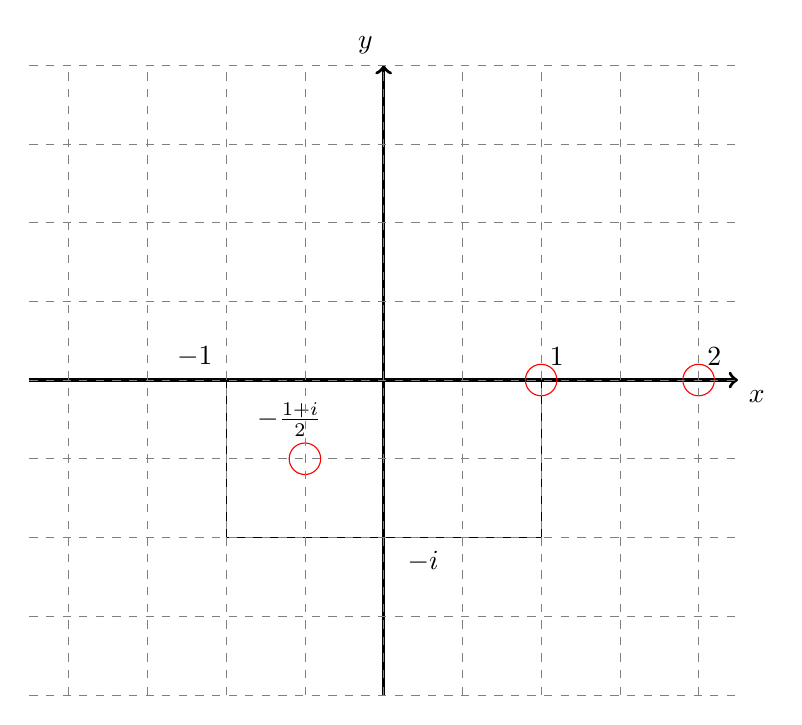
\begin{tikzpicture}
\draw[very thick,->] (-4.5,0) -- (4.5,0) node[anchor=north west] {$x$};
\draw[very thick,->] (0,-4) -- (0,4) node[anchor=south east] {$y$};
\draw[black](-2,0) -- (-2,-2) -- (2,-2) -- (2,0) -- (-2,0);

\draw[red] (2,0) circle (2mm) ;
\draw[red] (-1,-1) circle (2mm) ;
\draw[red] (4,0) circle (2mm) ;


\node at (0.5,-2.3) {$-i$};
\node at (2.2,0.3) {$1$};
\node at (-2.4,0.3) {$-1$};
\node at (4.2,0.3) {$2$};
\node at (-1.2,-0.5) {$-\frac{1+i}{2}$};

\draw[step=1cm,gray,dashed,very thin] (-4.5,-4) grid (4.5,4);
\end{tikzpicture}
\\
$$
\Rightarrow
I = \oint_{C_R} \frac{z-2i}{2\left(z+\frac{1+i}{2}\right)(z-2)(z-1)} dz
$$
\\
Θεωρούμε την $ f(z)=\frac{z-2i}{2\left(z+\frac{1+i}{2}\right)(z-2)(z-1)} ,\quad z\in\mathbb{C} -\left\{ 1,2, -\frac{1+i}{2} \right\}$
\\
$$
I=2\pi i Res\left(f,-\frac{1+i}{2}\right) + \frac{\pi i}{2} Res(f,1)
$$
Γενικά έχουμε ότι :

$$
\bullet\quad
Res\left(f,-\frac{1+i}{2}\right)= \lim_{z \rightarrow -\frac{1+i}{2}} \frac{z-2i}{2(z-2)(z-1)}=\frac{-\frac{1+i}{2}-2i}{2(-\frac{1+i}{2}-2)(-\frac{1+i}{2}-1)} 
$$
$$
\frac{-1-i-4i}{(-1-i-4)(-1-i-2)}=\frac{-(1+5i)}{(5+i)(3+i)}=\frac{-(1+5i)}{14+8i}=\frac{-(1+5i)(14-8i)}{14^2+8^2}=\frac{-54-62i}{250}
$$
$$
\bullet \quad
Res(f,1)=\lim_{z \rightarrow 1} \frac{z-2i}{(2z+1+i)(z-2)}
=\frac{1-2i}{(2+1+i)(1-2)}=\frac{-(1-2i)(3-i)}{10}=\frac{-1+7i}{10}
$$
$$\boxed{
I=2\pi i \frac{-54-62i}{250}  + \frac{\pi i}{2} \frac{-1+7i}{10}=\frac{\pi}{500}(73-241i)}
$$
 \subsection{Άσκηση 4}
$$f(z)={\sinh(\overline{z})} ,z=x+yi , x,y\in\mathbb{R}$$

$$f(z)=sinh(\overline{z})=\frac{e^{\overline{z}}-e^{-\overline{z}}}{2}=\frac{e^{x-yi}-e^{-(x-yi)}}{2}=
\frac{e^{x}e^{-yi}-e^{-x}e^{yi}}{2}
=$$
$$
=
\frac{e^{x}(cos(y)-isin(y))-e^{-x}(cos(y)+isin(y))}{2}=
\frac{cos(y)(e^{x}-e^{-x})-isin(y)(e^{x}+e^{-x})}{2}
=$$
\[
=
\underbrace{cos(y)sinh(x)}_{\text{$u(x,y)$}}-
\underbrace{sin(y)cosh(x)}_{\text{$v(x,y)$}}i
\]


$$u_x=cos(y)cosh(x)
$$
$$u_y=-sin(y)sinh(y)
$$
$$v_x=-sin(y)sinh(x)
$$
$$v_y=-cos(y)cosh(x)
$$


\[
\spalignsys {u_x=v_y;u_y=-v_x} \Rightarrow  
\spalignsys {cos(y)cosh(x)=-cos(y)cosh(x) ;
-sin(y)sinh(y)=sin(y)sinh(x)}
\Rightarrow 
\spalignsys
{cos(y)cosh(x)=0;
sin(y)sinh(y)=0} \Rightarrow
\]
\[
\Rightarrow
\spalignsys
{cos(y)=0;
sin(y)sinh(y)=0} \Rightarrow
\spalignsys
{y=\kappa \pi + \frac{\pi}{2}  {,}\quad \kappa \in \mathbb{Z};
sinh(x)=0} \Rightarrow
\]

\[
\spalignsys
{y=\kappa \pi + \frac{\pi}{2}  {,}\quad \kappa \in \mathbb{Z};
\frac{e^x-e^{-x}}{2}=0} 
\Rightarrow
\spalignsys
{y=\kappa \pi + \frac{\pi}{2}  {,}\quad \kappa \in \mathbb{Z};
e^{2x}=1}\Rightarrow
\spalignsys
{y=\kappa \pi + \frac{\pi}{2} {,}\quad \kappa \in \mathbb{Z};
x=0}
\]
Άρα η $f$ είναι παραγωγίσιμη στα σημεία $z_\kappa= i\left(\kappa \pi + \frac{\pi}{2} \right), \kappa\in\mathbb{Z} $ αλλά δεν είναι αναλυτική , αφού δεν υπάρχουν σημεία που είναι παραγωγίσιμη σε αυτά αλλά και σε όλα τα σημεία σε έναν ανοικτό δίσκο γύρω τους για οσοδήποτε
μικρή ακτίνα (είναι παραγωγίσιμη σε διακριτά σημεία).
\newpage
 \subsection{Άσκηση 5}
$$f(z)= \frac{cos(\pi z)(e^{-2z} - (z+1)^2 +4z)}{z^3(2z+1)^2}
$$
$\bullet \quad $πόλος στο $ζ_0=0$ πρώτης τάξης.\\
$\bullet \quad $πόλος στο $ζ_1=-\frac{1}{2}$ πρώτης τάξης.

$$
\bullet \quad \lim_{z \rightarrow 0} \frac{e^{-2z} - (z+1)^2 +4z}{z^2}
\overset{\mathrm{(\frac{0}{0})DLH}}{=\joinrel=\joinrel=\joinrel=}
\lim_{z \rightarrow 0} \frac{-2e^{-2z} - 2(z+1)+4}{2z}
\overset{\mathrm{(\frac{0}{0})DLH}}{=\joinrel=\joinrel=\joinrel=}
\lim_{z \rightarrow 0} \frac{4e^{-2z}- 2}{2}=1
$$
$$
\bullet \quad \lim_{z \rightarrow 0} \frac{cos(\pi z)}{(2z+1)^2}=-1
$$
Άρα $$
\lim_{z \rightarrow 0} zf(z)=1 =Res(f,0)
$$

$$\bullet \quad \lim_{z \rightarrow -\frac{1}{2}}
\frac{cos(\pi z)(e^{-2z} - (z+1)^2 +4z)\cancel{(z+\frac{1}{2})}}{4z^3(z+\frac{1}{2})\cancel{^2}}=(2e-6)\pi=Res(f,-\frac{1}{2})
$$
$$
\bullet \quad \lim_{z \rightarrow 0} \frac{cos(\pi z)}{(z+\frac{1}{2})}\overset{\mathrm{DLH}}{=\joinrel=} 
\lim_{z \rightarrow 0} -\pi sin(\pi z) =-\pi
$$

$$\bullet \quad \lim_{z \rightarrow -\frac{1}{2}}
\frac{(e^{-2z} - (z+1)^2 +4z)}{4z^3}=\frac{e-1/4-2}{-1/2}=6-2e
$$
 \subsection{Άσκηση 6}
$Lauren $ γύρω από το $z_0=0 , 1<|z|<3$
$$
f(z)=\frac{z-5i}{z^2-2iz+3}=\frac{z-5i}{(z-3i)(z+i)}=
=\frac{3}{2(z+i)}-\frac{1}{2(z-3i)}
$$
$$=
\frac{3/2}{z(1+\frac{i}{z}}+\frac{1/2}{3i(1-\frac{z}{3i}}=
\frac{3}{2z}\sum_{n=0}^{+\infty}\left(\frac{-i}{z}\right)^n-\frac{1}{6i}\sum_{n=0}^{+\infty}\left(\frac{z}{3i}\right)^n ,\quad 1<|z|<3
$$
\newpage
 \subsection{Άσκηση 7}
Η $f$ είναι αναλυτική στο $D$ και σταθερή πάνω στον κύκλο 
$|z|=r< R ,$\\$ \quad D= \{ z \in \mathbb{C} : |z| < R \}$.
\\ \\
Η $f$ είναι συνεχής στο σύνορο του κύκλου $|z|=r$. Από το θεώρημα μεγίστου η $|f(z)|$ θα έχει μέγιστο στο $\partial{E}$ , $\quad |f(z)|\leq M$.
\\
Από το θεώρημα $Liouville$ (αφού είναι φραγμένη και αναλυτική ) θα είναι σταθερή στο Ε.
\\ \\
Όμοια η $f$ θα έχει μέγιστο στο $D-E$ ,πάνω στο σύνορο $\partial{E}$ και άρα είναι σταθερή στο $D-Ε$.
\\ \\
Συνεπώς, η $f$ είναι σταθερή στο $D$.

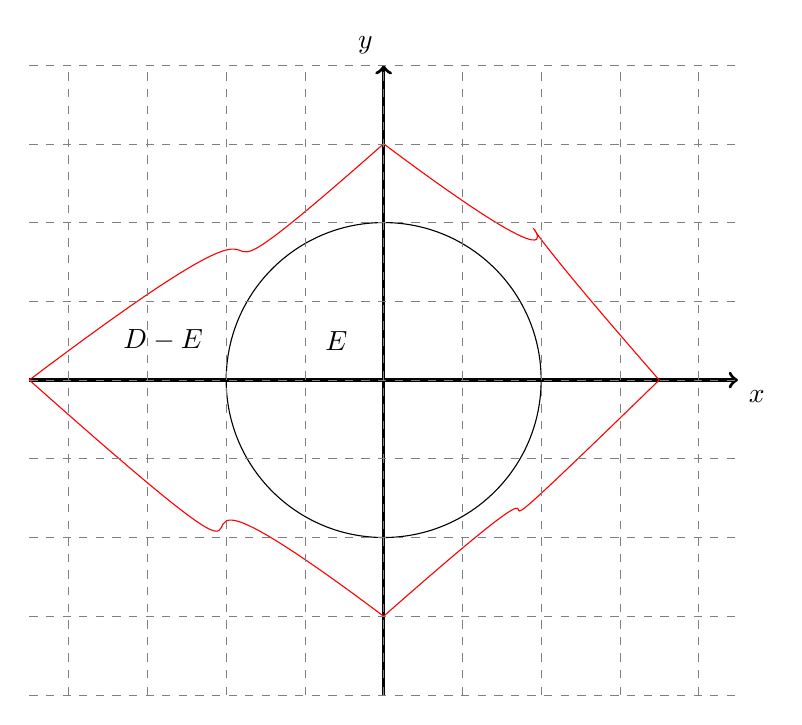
\begin{tikzpicture}
\draw[very thick,->] (-4.5,0) -- (4.5,0) node[anchor=north west] {$x$};
\draw[very thick,->] (0,-4) -- (0,4) node[anchor=south east] {$y$};

\draw[black] (0,0) circle (2cm) ;
\draw[red] (3.5,0) .. controls (0,4) and (4,0) .. (0,3);
\draw[red] (3.5,0) .. controls (0,-3.4) and (3.4,0) .. (0,-3);
\draw[red] (-4.5,0) .. controls (0,-4) and (-4,0) .. (0,-3);
\draw[red] (-4.5,0) .. controls (0,3.4) and (-3.4,0) .. (0,3);

\node at (-0.6,0.5) {$E$};
\node at (-2.8,0.5) {$D-E$};

\draw[step=1cm,gray,dashed,very thin] (-4.5,-4) grid (4.5,4);
\end{tikzpicture}
\newpage
 \subsection{Άσκηση 8}
$$I= \int_{-\infty}^{+\infty} \frac{dx}{(x-1)(x^2+4)^2}$$
\\
Θέτουμε $ f(z)=\frac{1}{(z-1)(z^2+4)^2},z\in\mathbb{C}-\{-2i,2i,1\} $. Έχουμε τρεις πόλους,έναν πρώτης τάξης,
πάνω στον πραγματικό άξονα$(z_3=1) $ και δύο δεύτερης τάξης,έναν στο άνω$(z_1=2i)$ και  έναν στο κάτω ημιεπίπεδο$(z_2=-2i)$.

$$ \lim_{z \to \infty } zf(z)=\lim_{z \to \infty } \frac{z}{(z-1)(z^2+4)^2}=
\lim_{z \to \infty } \frac{z}{z\left(1-\frac{1}{z}\right)(z^2+4)^2}=
\lim_{z \to \infty } \frac{1}{\left(1-\frac{1}{z}\right)(z^2+4)^2}=0$$

Επομένως $$ Ι= 2 \pi i Res(f,2i)+ \pi i Res(f,1)\quad (1) $$

$$\bullet \quad Res(f,1)=\lim_{z\to 1}\frac{\cancel{z-1}}{\cancel{(z-1)}(z^2+4)^2}=\lim_{z\to 1}\frac{1}{(z^2+4)^2}=\frac{1}{25}=\frac{16}{400}$$

$$\bullet \quad 
Res(f,2i)=\lim_{z\to 2i} \left[ \frac{\cancel{(z-2i)^2}}{(z-1)(z+2i)^2\cancel{(z-2i)^2}} \right]'= 
\lim_{z\to 2i} 
\frac{-(z+2i)^2-2(z-1)(z+2i)}{(z-1)^2(z+2i)^4}=
$$
$$=
\frac{-(4i)^2+(1-2i)(4i)}{(1-2i)^2(4i)^2}
=\frac{-13-16i}{(2i)400}
$$
\\
Άρα η $(1)$ γίνεται:
\\
$$ Ι=\pi  \left[ \frac{-13-16i}{400} \right] + \pi i \left( \frac{16}{400} \right) = 
-\frac{13\pi}{400}
$$
\\
Άρα $$ \int_{-\infty}^{+\infty} \frac{dx}{(x-1)(x^2+4)}= -\frac{13\pi}{400} $$

 

\newpage \part{Εφαρμοσμένα Μαθηματικά Φεβρουάριος 2014}
\author{}
  

\maketitle
\newpage
 

 \section{Θέματα Ατρέα}
 \subsection{Άσκηση 1}
(α) $$z^6=(-i)^{-i}=e^{-ilog(-i)}=e^{-i[ln(|-i|)+i(-\frac{\pi}{2}+2 \kappa \pi)]}=e^{\pi\left(2\kappa -\frac{1}{2}\right)}\Rightarrow
$$
$$\Rightarrow
z=\sqrt[6]{|e^{\pi\left(2\kappa -\frac{1}{2}\right)}|}e^{\frac{2\lambda\pi i}{6}}
=\sqrt[6]{e^{\pi\left(2\kappa -\frac{1}{2}\right)}}e^{\frac{\lambda\pi i}{3}}$$
με $\kappa\in \mathbb{Z},\lambda={0,1,2,3,4,5}$ 
\\
Άρα

\[
z= 
\spalignsys{
\sqrt[6]{e^{\pi\left(2\kappa -\frac{1}{2}\right)}};
\sqrt[6]{e^{\pi\left(2\kappa -\frac{1}{2}\right)}} ( \frac{\sqrt{3}+i}{2} );
\sqrt[6]{e^{\pi\left(2\kappa -\frac{1}{2}\right)}} ( \frac{-\sqrt{3}+i}{2} );
-\sqrt[6]{e^{\pi\left(2\kappa -\frac{1}{2}\right)}} ;
\sqrt[6]{e^{\pi\left(2\kappa -\frac{1}{2}\right)}} ( \frac{-\sqrt{3}-i}{2} );
\sqrt[6]{e^{\pi\left(2\kappa -\frac{1}{2}\right)}} ( \frac{\sqrt{3}-i}{2} )
 }
 \quad,\kappa \in \mathbb{Z}
\]
\\
(β) Παραμετροποίηση
$$ \gamma_1(t)=z_1+t(z_1-z_2) \quad ,t\in[0,1]$$
$$ \gamma_2(t)=z_3+t(z_3-z_4) \quad ,t\in[0,1]$$
Για να είναι παράλληλες οι $ \gamma_1(t),\gamma_2(t)$ πρέπει:
$$ (z_1-z_2)= (z_3-z_4) \Leftrightarrow \frac{z_1-z_2}{z_3-z_4}=1\in\mathbb{R}
  \Leftrightarrow Im \left(\frac{z_1-z_2}{z_3-z_4}\right)=0 $$
\newpage
 \subsection{Άσκηση 2}

Ο γεωμετρικός τόπος των σημείων $z$ του επιπέδου, η διανυσματική ακτίνα των οποίων, σχηματίζει γωνία $-\frac{\pi}{4}$ ή $\frac{3\pi}{4}$  με τον ημιάξονα $Ox$. Δηλαδή η ευθεία $y=x$

$$ f(z)=1 - \frac{2}{z-i} , \quad z \in \mathbb{C}-\{i\}$$

Θέτουμε $ z=x+yi $ και $y=-x$ έχουμε:

$$ f(x+yi)=1-\frac{2}{x-i(x+1)}=1-\frac{2[x+i(x+1)]}{x^2+(x+1)^2}=1-\frac{2x}{x^2+(x+1)^2} -i \frac{2(x+1)}{x^2+(x+1)^2} $$
 
Θέτουμε 

\[
\spalignsys{
u(x{,}y)= 1-\frac{2x}{x^2+(x+1)^2} ; ; v(x{,}y)= -\frac{2(x+1)}{x^2+(x+1)^2}
 } \Rightarrow
 \spalignsys{
\frac{1-u}{2}= \frac{x}{x^2+(x+1)^2} \quad (1); ; v= -\frac{2(x+1)}{x^2+(x+1)^2 }\quad (2)
 } 
  \]
$$ (2),(1) \overset{(:)}{\Longrightarrow} \frac{2v}{1-u}= -\frac{2(x+1)}{x} \Rightarrow \frac{v}{u-1}= 1+\frac{1}{x} \Rightarrow x= \frac{u-1}{v-u+1} $$ 
 \\
 Αντικαθιστόντας την παραπάνω σχέση στη $(2)$ έχουμε:
 
$$ v=-\frac{2\left(\frac{u-1}{v-u+1} +1\right)}{\left( \frac{u-1}{v-u+1} \right)^2+\left(\frac{u-1}{v-u+1} +1 \right)^2} \Rightarrow 
v= -\frac{2\left(\frac{v}{v-u+1}\right)}{ \frac{(u-1)^2+v^2}{(v-u+1)^2}} 
\Rightarrow
(u-1)^2+v^2=-2(v-u+1)
\Rightarrow
$$ 
 $$ \Rightarrow u^2-2u+1+v^2+2v-2u+4=-2+4 \Rightarrow  u^2-4u+4+v^2+2v+1=2 \Rightarrow$$
 $$  \Rightarrow (u-2)^2+(v+1)^2=(\sqrt{2})^2 $$

Κύκλος με κέντρο το $Κ(2,-1)$ και ακτίνα $r=\sqrt{2}$ 
\\ \\
Το παραπάνω ισχύει όταν $u\neq 1$.
Αν $u=1,\quad (1)\Rightarrow x=0, \quad (2) \Rightarrow v=-2$, δηλαδή το σημείο $Α=(1,-2)$ το οποίο ανήκει στον παραπάνω κύκλο, άρα ισχύει σε κάθε περίπτωση.
\\ \\
 
 \newpage
 \subsection{Άσκηση 3}

$$ f(z)=\frac{2\sinh^2(z)-4z^2}{z(z^3-2z^2-3z)}=\frac{2\sinh^2(z)-4z^2}{z^2(z-3)(z+1)},z\in\mathbb{C}-\{-1,0,3\}$$

\begin{enumerate}

\item
$$ \lim_{z\to 0}f(z)=  \frac{2}{3}\in\mathbb{C} \quad $$ απαλείψιμη ανωμαλία, δηλαδή
$$ Res(f,0)=0 $$
αφού
$$ \bullet \quad \lim_{z\to 0}\frac{2\sinh^2(z)-4z^2}{z^2}\overset{\mathrm{De L'Hospital}}{=\joinrel=\joinrel=\joinrel=\joinrel=\joinrel=\joinrel=}
\lim_{z\to 0}\frac{4\sinh(z)\cosh(z)-8z}{2z}\overset{\mathrm{De L'Hospital}}{=\joinrel=\joinrel=\joinrel=\joinrel=\joinrel=\joinrel=}$$ 
$$=\lim_{z\to 0}\frac{4\cosh^2(z)+4\sinh^2(z)-8}{2}=-2$$

$$ \bullet \quad \lim_{z\to 0} \frac{1}{(z-3)(z+1)}=-\frac{1}{3} $$

\item
$$ Res(f,-1)= \lim_{z\to -1}f(z)=\lim_{z\to -1}\frac{(z+1)(2\sinh^2(z)-4z^2)}{z^2(z-3)(z+1)} =$$
$$=\lim_{z\to -1}\frac{2\sinh^2(z)-4z^2}{z^2(z-3)}=\frac{2\sinh^2(-1)-4}{(-4)} $$ πόλος πρώτης τάξης

\item
$$ Res(f,3)= \lim_{z\to 3}f(z)=\lim_{z\to 3}\frac{(z-3)(2\sinh^2(z)-4z^2)}{z^2(z-3)(z+1)}= $$
$$=\lim_{z\to 3}\frac{2\sinh^2(z)-4z^2}{z^2(z+1)}=\frac{2\sinh^2(-1)-4}{36} $$ πόλος πρώτης τάξης

\end{enumerate}

\newpage
 \subsection{Άσκηση 4}

(α) Η $f(z)=f(x+yi)=u(x,y)+iv(x,y)$ είναι ακέραια ( δηλαδή αναλυτική στο $\mathbb{C}$) με 
$$ u(x,y)=(x^3+y^3) \quad,\quad v(x,y)=(x^2-y^2) $$
\\
Από τις εξισώσεις $Cauchy-Riemann$ έχουμε
\\
\[
\spalignsys {u_x=v_y;u_y=-v_x} \Rightarrow \spalignsys {3x^2+2y=0 ; 3y^2-2x=0} \Rightarrow
\spalignsys { 3\left(\frac{3y^2}{2}\right)^2+2y=0 ; x=\frac{3y^2}{2}} \Rightarrow 
\spalignsys { 27y^4+8y=0 ; x=\frac{3y^2}{2}} \Rightarrow 
\]
\[\Rightarrow
\spalignsys { y(27y^3+8)=0 ; x=\frac{3y^2}{2}} \spalignsys { y=0 \quad $ή$ \quad y=-\frac{2}{3} ; x=\frac{3y^2}{2} \quad (1)}
\]
\\
Για $y=0, \quad (1)\Rightarrow x=0$ \\
Για $y=-\frac{2}{3}, \quad (1)\Rightarrow x=\frac{2}{3} $
\\ \\
Άρα η $f$ είναι παραγωγίσιμη στα σημεία $z=0$ και $z=\frac{2}{3}(1-i)$.
\\ \\
(β)
Η $f$ δεν είναι αναλυτική , αφού δεν υπάρχουν σημεία που να είναι παραγωγίσιμη σε αυτά αλλά και σε όλα τα σημεία σε έναν ανοικτό δίσκο γύρω τους για οσοδήποτε μικρή ακτίνα.
\\ \\
(γ)
$$ I= \int_\gamma f(z)dz, \quad \gamma:y=2x^2,x\in[1,2] $$
Παραμετροποίηση:
$$ z(t)=x(t)+iy(t)=t+2it^2,t\in[1,2] $$
$$ I= \int_\gamma f(z)dz= \int_{1}^{2} f(x(t)+iy(t))\frac {d(x(t)+iy(t))}{dt} dt = $$ 
$$= \int_{1}^{2} [(x^3(t)+y^3(t))+i(x^2(t)-y^2(t))]\frac {d(x(t)+iy(t))}{dt} dt= $$
$$= \int_{1}^{2} [(t^3+8t^6)+i(t^2-4t^4)](1+4it) dt= $$
$$= \int_{1}^{2} (t^3+8t^6+it^2-4it^4+4it^4+32it^7-4t^3+16t^5) dt= $$
$$= \left[\frac{t^4}{4}+\frac{8t^7}{7}-t^4+\frac{8t^6}{3}\right]^{2}_{1}+
i\left[\frac{t^3}{3}+4t^8 \right]^{2}_{1}= \frac{8453}{28}+i\frac{3067}{3}$$

\newpage
 \subsection{Άσκηση 5}
$$Ι=\oint_{C} \frac{z^2-1}{z}\cos{\left(\frac{2}{z}\right)} dz ,\quad C:|z|=3$$

Θεωρούμε την  $f(z)=\frac{z^2-1}{z}\cos{\left(\frac{2}{z}\right)},z\in\mathbb{C}-\{0\}$.
\\ \\
Γενικά έχουμε ότι :
$$\bullet \quad \frac{z^2-1}{z}=z-\frac{1}{z}$$ 
$$\bullet \quad \cos{\left(\frac{2}{z}\right)} =\sum_{n=0}^\infty \frac{(-1)^n}{(2n)!}\left(\frac{2}{z}\right)^{2n} $$ 
Άρα : 
$$ f(z)=\left(z-\frac{1}{z} \right)\left[ \sum_{n=0}^\infty \frac{(-1)^n}{(2n)!}\left(\frac{2}{z}\right)^{2n} \right]= $$
$$ = \left(z-\frac{1}{z} \right)\left( 1-\frac{2^2}{2!z^2}+\frac{2^4}{4!z^4}-\frac{2^6}{6!z^6} +\ldots \right) = \left( z-\frac{1}{z}-\frac{2^2}{2!z}+\frac{2^4}{4!z^3}+\frac{2^4}{4!z^5} -\ldots \right) $$
\\
Συνεπώς:
$$
Res(f,0)=-1+\frac{2^2}{2!}=-3$$
Άρα : $$ Ι=2\pi i Res(f,0) = -6 \pi i $$
\newpage

 \subsection{Άσκηση 6}
$$
A,B > 0  \qquad |f(z)|\leqslant A|z|+B,\forall z \in \mathbb{C}
$$
Αν $f$ πολυώνυμο το πολύ 1ου βαθμού 
$f(z)=az+b,\quad a,b\in \mathbb{C}$ τότε 
$f'(z)=a,\quad f''(z)=0$
\\ \\
Έχουμε ότι : $|f^{(n)}(z)|\leqslant \frac{n!M_r}{R^n}$ και 
\[
M_r=max\{|f(z)|:
\underbrace{|z-z_o|=R}_{\text{$z=z_o+Re^{i\theta}$}}
\}
\]
\\
Αρκεί να δείξουμε ότι: $f''(z)=0,\forall z \in \mathbb{C}$
$$
|f(z)|\leqslant A|z|+B=A|z_o+Re^{i\theta}|+B
\leqslant A|z_o|+AR|e^{i\theta}|+B=
AR+A|z_o|+B
\Rightarrow$$
$$\Rightarrow
|f''(z)|\leqslant\frac{2!(AR+A|z_o|+B)}{R^2}
\overset{\mathrm{R\rightarrow +\infty}}{\Rightarrow} $$
$$ \Rightarrow |f''(z)|\leqslant0 \Rightarrow f''(z)=0$$

\newpage
 \subsection{Άσκηση 7}
$$
I=\int_{0}^{2\pi} \frac{\cos{(2 \theta)}}{\sqrt{5}+\sin{(\theta)}} d \theta=\int_{0}^{2\pi} \frac{2\cos^2{(\theta)}-1}{\sqrt{5}+\sin{(\theta)}} d \theta
$$  \\
Θέτουμε $z=e^{i\theta}\Rightarrow dz=ie^{i\theta}d\theta \Rightarrow \frac{dz}{iz}=d\theta \quad$ και ολοκληρώνουμε πάνω στην καμπύλη $|z|=1$
$$ \cos(\theta)=\frac{e^{i\theta}+e^{-i \theta}}{2}=\frac{1}{2} \left( z + \frac{1}{z} \right) $$
$$ \sin(\theta)=\frac{e^{i\theta}-e^{-i \theta}}{2i}=\frac{1}{2i} \left( z - \frac{1}{z} \right) $$
Άρα 
$$ Ι= \oint_{|z|=1}^{ } \frac{\frac{1}{2}\left( z + \frac{1}{z} \right)^2-1}{\sqrt{5}+\frac{1}{2i} \left( z - \frac{1}{z} \right)} \frac{dz}{iz} = 
\oint_{|z|=1}^{ } \frac{\left( z + \frac{1}{z} \right)^2-2}{2\sqrt{5}iz+z \left( z - \frac{1}{z} \right)} dz =
\oint_{|z|=1}^{ } \frac{ z^2 + \frac{1}{z^2} }{2\sqrt{5}iz+z^2-1} dz = $$

$$ =\oint_{|z|=1}^{ } \frac{ z^4 + 1 }{z^2(z^2+2\sqrt{5}iz-1)} dz $$

Λύνουμε $z^2(z^2+2\sqrt{5}iz-1)=0 \Rightarrow z=0\quad$ ή
$$\quad z^2+2\sqrt{5}iz-1=0 $$
$$ \Delta=-20+4=-16 \qquad z_{1,2}=\frac{-2\sqrt{5}i\pm 4i}{2} \Rightarrow \spalignsys{z_1=(2-\sqrt{5})i;z_2=(-2-\sqrt{5})i} $$ 
Άρα 
$$ Ι=\oint_{|z|=1} \frac{ z^4 + 1 }{z^2(z-(2-\sqrt{5})i)(z+(2+\sqrt{5})i)} dz $$
\\
Θέτουμε $f(z)=\frac{ z^4 + 1 }{z^2(z-(2-\sqrt{5})i)(z+(2+\sqrt{5})i)},\quad z\in\mathbb{C}-\{0,(2-\sqrt{5})i,(-2-\sqrt{5})i\} $
\\ \\
Η $f$ έχει τρείς πόλους.
\begin{itemize}
\item $z_0=0$ ,διπλός πόλος
\item $z_1=(2-\sqrt{5})i$ ,απλός πόλος
\item $z_2=(-2-\sqrt{5})i$ ,απλός πόλος (δεν ανήκει στον κύκλο $|z|=1$)
\\
\end{itemize}

Άρα $I=2\pi i \left[ Res(f,z_0)+ Res(f,z_1) \right] \quad (1)$
\\
$$ \bullet\quad Res(f,z_0)=\lim_{z \to 0}\left[\frac{\cancel{z^2}(z^4+1)}{\cancel{z^2}(z-z_1)(z-z_2)}\right]'=$$
$$ =\lim_{z \to 0}\left[\frac{ 4z^3(z-z_1)(z-z_2)-(z^4+1)((z-z_2)+(z-z_1))}{ (z-z_1)^2(z-z_2)^2}\right]=\frac{ z_1+z_2}{ z_1^2 z_2^2}=$$
$$ =\frac{-2\sqrt{5}i}{(2-\sqrt{5})^2(2+\sqrt{5})^2}= -2\sqrt{5}i = \frac{4\sqrt{5}}{2i} $$



$$ \bullet\quad Res(f,z_1)=\lim_{z \to z_1}\left[\frac{\cancel{(z-z_1)}(z^4+1)}{z^2\cancel{(z-z_1)}(z-z_2)}\right]=\frac{z_1^4+1}{z_1^2(z_1-z_2)}=$$
$$= \frac{(2-\sqrt{5})^4+1}{(2-\sqrt{5})^2(-4i)}=-\frac{(2-\sqrt{5})^2}{2(2i)}-\frac{1}{2(2-\sqrt{5})^2(2i)}=$$
$$=-\frac{(2-\sqrt{5})^2}{2(2i)}-\frac{(2+\sqrt{5})^2}{2(4-5)^2(2i)}=-\frac{(2-\sqrt{5})^2+(2+\sqrt{5})^2}{2(2i)}=$$
$$ =-\frac{4-2\sqrt{5}+5+4+2\sqrt{5}+5}{2(2i)}=-\frac{9}{2i} $$

Έτσι η $(1)$ γίνεται:
$$ I=2\pi i \left[ \frac{4\sqrt{5}}{2i} -\frac{9}{2i} \right]= (4\sqrt{5}-9)\pi $$

Άρα 
$$I=\int_{0}^{2\pi} \frac{\cos{(2 \theta)}}{\sqrt{5}+\sin{(\theta)}} d \theta=  (4\sqrt{5}-9)\pi $$
 

\newpage \part{Εφαρμοσμένα Μαθηματικά Σεπτέμβριος 2013}
\author{}


  

\maketitle
\newpage
 

 \section{Θέματα Ατρέα}
 \subsection{Άσκηση 1}

(α) 
$$ \gamma : \left\{ z=x+yi, \quad Im \overline{\left( \frac{z}{(1-i)^5} \right)}=2  \right\} $$

$$ \overline{ \left( \frac{z}{(1-i)^5} \right)}= \frac{\overline{z} }{(1+i)^5 }= \frac{\overline{z} }{(1+i)^2(1+i)^2(1+i) }= \frac{x-yi }{(2i)^2(1+i) }= $$

$$ = \frac{ (x-yi)(1-i) }{(-8) }=\frac{ (y-x)+(x+y)i }{8} $$

Άρα

$$ Im \overline{\left( \frac{z}{(1-i)^5} \right)}=2 \Rightarrow \frac{ x+y }{8}=2 \Rightarrow y=-x+16 $$

$$ w=-\frac{32}{z} \Rightarrow w=-\frac{32 \overline{z}}{|z|^2} \Rightarrow w=-\frac{32x}{x^2+y^2}+i\frac{32y}{x^2+y^2} $$
\\
Θέτουμε $w=u(x,y)+iv(x,y), \quad $ άρα $\quad u(x,y)=-\frac{32x}{x^2+y^2} \quad $  και $\quad v(x,y)= \frac{32y}{x^2+y^2}$

\[ 
\spalignsys{u=-\frac{32x}{x^2+y^2} ; ; v=\frac{32y}{x^2+y^2}}
\overset{y=-x+16}{\Longrightarrow}
\spalignsys{u=-\frac{32x}{x^2+(x-16)^2} \quad (1) ; ; v=-\frac{32(x-16)}{x^2+(x-16)^2}\quad(2)}
\] 

$$ (1),(2)\Rightarrow \frac{v}{u}= \frac{x-16}{x}\Rightarrow \frac{v}{u}= 1-\frac{16}{x} \Rightarrow 1-\frac{v}{u}= \frac{16}{x}\Rightarrow x= \frac{16u}{u-v}$$
Άρα
$$ (1)\Rightarrow u= \frac{\left(-\frac{32\cdot16u}{u-v} \right)}{\left( \frac{16u}{u-v}\right)^2+\left( \frac{16u}{u-v} -16 \right)^2}
\Rightarrow u= \frac{\left(-\frac{32\cdot16u}{u-v} \right)}{  \frac{(16u)^2+(16u-16(u-v))^2}{(u-v)^2}} \Rightarrow $$

$$ \Rightarrow u= \frac{(u-v)(-32\cdot16u)}{(16u)^2+(16v)^2} \Rightarrow 16^2u(u^2+v^2)= 2\cdot16^2u(v-u) \Rightarrow u^2+v^2= 2(v-u) \Rightarrow $$

$$ \Rightarrow u^2+2u +v^2-2v + 2 = 2 \Rightarrow (u+1)^2 + (v-1)^2 = \sqrt{2}^2 $$
Κύκλος με κέντρο το $Κ(-1,1)$ και ακτίνα $r=\sqrt{2}$ 
\\ \\
Το παραπάνω ισχύει όταν $u\neq 0$.
Αν $u=0,\quad (1)\Rightarrow x=0, \quad (2) \Rightarrow v=2$, δηλαδή το σημείο $Α=(0,2)$ το οποίο ανήκει στον παραπάνω κύκλο, άρα ισχύει σε κάθε περίπτωση.
\\ \\
(β)
Αφού $a\in\mathbb{C}-\{0\}$ έχουμε:
$$ a^{-N}=\left( |a|e^{i\theta} \right)^{-N}= |a^{-N}|e^{i(-N\theta)} $$
Θέτοντας $ s=a^{-N},\quad s\in\mathbb{C}-\{0\}\quad $ έχουμε $|s|=|a^{-N}|=|a|^{-N} \quad$ και 
\\  
$\quad Arg(s)=-N\theta $
\\ \\
Άρα:
$$ \sqrt[N]{a^{-N}}= \sqrt[N]{s}=\sqrt[N]{|s|}e^{i\left(\frac{Arg(s)+2\kappa\pi}{N}\right)}=\sqrt[N]{|a|^{-N}}e^{i\left(\frac{-N\theta+2\kappa\pi}{N}\right)}, \quad \kappa=0,1,2,...,N-1 $$
\\
Άρα:
$$ \sqrt[N]{a^{-N}}=|a|^{-1}e^{-i\theta}e^{i\left(\frac{2\kappa\pi}{N}\right)} =\left(|a|e^{i\theta}\right)^{-1}e^{i\left(\frac{2\kappa\pi}{N}\right)}=a^{-1}e^{\frac{2\kappa\pi i}{N}}, \quad \kappa=0,1,2,...,N-1 $$

\newpage
 \subsection{Άσκηση 2}
(α) Θέτουμε $f(x+yi)=u(x,y)+iv(x,y)$ , άρα $\overline{f(x+yi)}=u(x,y)-iv(x,y)$
\\ \\
Από τις εξισώσεις $ Cauchy-Riemann $ για την $f$ έχουμε:
\[
\spalignsys {u_x=v_y \quad (1) ; u_y=-v_x \quad (2)}
\]
Από τις εξισώσεις $ Cauchy-Riemann $ για την $\overline{f}$ έχουμε:
\[
\spalignsys {u_x=-v_y \quad (3); u_y=v_x\quad (4)}
\]
$$ (1),(3)\overset{(+)}{\Longrightarrow}2u_x=0\Rightarrow u_x=0=v_y $$
$$ (2),(4)\overset{(+)}{\Longrightarrow}2u_y=0\Rightarrow u_y=0=v_x $$
\\
Άρα $f'(z)=f_x=u_x+iv_x=0\Rightarrow f(z)=c,\quad c\in\mathbb{C}$
\\ \\ 
(β)
\\
$ P(z)=e^{Az+B}, \quad A,B\in\mathbb{C} $\\
$ P'(z)=Ae^{Az+B} $\\
$ 0<Im(B)<2\pi \quad (5)$\\

Το σημείο $ z=-i \quad$ βρίσκεται εντός της καμπύλης $\gamma : |z-1|=3$
\\
Επομένως, από τον ολοκληρωτικό τύπο του $Cauchy$ για παραγώγους έχουμε:
$$ P(-i)=\frac{1}{2\pi i} \int_\gamma \frac{P(z)}{z+i}=\frac{2\pi^2 i}{2\pi i}=\pi $$
$$ P'(-i)=\frac{1}{2\pi i} \int_\gamma \frac{P(z)}{(z+i)^2}=\frac{2\pi^3 i}{2\pi i}=\pi^2 $$
\\
\[
\spalignsys {e^{-Ai+B}=\pi ;Ae^{-Ai+B}=\pi^2}
\Rightarrow
\spalignsys {e^{-Ai+B}=\pi ;A=\pi}
\Rightarrow
\spalignsys {e^{-i\pi+B}=\pi ;A=\pi}
\Rightarrow
\spalignsys {e^{B}=-\pi ;A=\pi}
\Rightarrow
\]

\[
\Rightarrow
\spalignsys {B=\log(-\pi) ;A=\pi}
\Rightarrow
\spalignsys {B=\ln|-\pi| + i ( \pi + 2\kappa \pi ) {,} \kappa\in\mathbb{Z} ; A=\pi}
\overset{(5)}{\Longrightarrow}
\spalignsys {A=\pi ; B=\ln(\pi) + i  \pi }
\]
\\ \\
(γ) 
$$ Ι=\int_{c}|P(z)|dz=\int_{c}|e^{\pi z+\ln(\pi)+i \pi}|dz=\pi\int_{c}|e^{\pi Re(z)+i\pi(Im(z)+1)}|dz=\pi\int_{c}e^{\pi Re(z)}dz$$

Παραμετροποίση ευθυγράμμου τμήματος $c$:
$$ \gamma(t)=(1-i)+t[(2+4i)-(1-i)]=(1+t)+i(5t-1),\quad t\in[0,1] $$
$ \qquad \gamma'(t)=1+5i $
\\ \\
Αν $g(z)=e^{\pi Re(z)} ,z\in\mathbb{C} $ τότε:
$$ Ι=\int_{c}g(z)dz=\int_{c}g(\gamma(t))\gamma'(t)dt= \int_{0}^{1} \pi e^{\pi (t+1) }(1+5i)dt=(1+5i)\left[e^{\pi (t+1) }\right]_{0}^{1}\Rightarrow$$
$$\Rightarrow I=(1+5i)(e^{2\pi}-e^{\pi}) $$




 \newpage
 \subsection{Άσκηση 3}
(α)
Έστω ότι η $f$ δεν έχει ρίζα  στο εσωτερικό του $ D ,\quad f(z)\neq 0, \forall z \in D$.
\\ \\
Αφού η $f$ είναι αναλυτική σε όλο το $D$, άρα είναι και συνεχής στο σύνορο $\partial D$ και $|f(z)|\neq0$, θα ισχύει το Θεώρημα Ελαχίστου.
\\ \\
Επομένως η $|f(z)|$ παίρνει ελάχιστο πάνω στο σύνορο $\partial D$.
\\ \\
Όμως $|f(z_0)|=2<3$ το οποίο είναι ΑΤΟΠΟ αφού $ |f(z)|\geq 3,\forall z \in \partial D$. 
\\ \\
 Άρα $|f(z)|=0\Rightarrow f(z)= 0$ για ένα τουλάχιστον $z$ στο εσωτερικό του $D$
\\ \\
(β)

$$ f(z)= (2z-1)\cos{\left(\frac{1}{z+1}\right)} , z \in \mathbb{C}- \{ -1 \} $$


Γενικά έχουμε ότι :
$$\bullet \quad (2z-1)=2(z+1)-3$$
 
$$\bullet \quad \cos{\left(\frac{1}{z+1}\right)} =\sum_{n=0}^\infty \frac{(-1)^n}{(2n)!}\left(\frac{1}{z+1}\right)^{2n} $$ 

Άρα : 
$$ f(z)=[2(z+1)-3]\left[ \sum_{n=0}^\infty \frac{(-1)^n}{(2n)!}\left(\frac{1}{z+1}\right)^{2n} \right]= $$
$$= [2(z+1)-3] \left( 1-\frac{1}{2!(z+1)^2}+\frac{1}{4!(z+1)^4}-\frac{1}{6!(z+1)^6}+...  \right)=  $$
$$=  2(z+1)-\frac{2}{2!(z+1)}+\frac{2}{4!(z+1)^3}-\frac{2}{6!(z+1)^5}+...-3+  \frac{3}{2!(z+1)^2}-\frac{3}{4!(z+1)^4}+\frac{3}{6!(z+1)^6}+... $$
\\
Συνεπώς:
$$ Res(f,-1)=-\frac{2}{2!}=-1 $$

\newpage
 \subsection{Άσκηση 4}
(α)
$$ Ι=\oint_{\gamma} \frac{ e^z(\cos(z)-1)}{\sin^2(z)(3z+i)}dz $$
\\ \\
Λύνουμε 
$$\sin^2(z)(3z+i)=0 \Rightarrow \sin(z)=0 \Rightarrow $$

\[
\spalignsys{z=2\kappa \pi ; z=2 \kappa \pi +\pi}{,}\kappa\in\mathbb{Z}
\quad \Rightarrow z_1=0,\quad z_1\in\gamma
\]
ή 
$$3z+i=0\Rightarrow z_2=-\frac{i}{3},\quad z_2\in\gamma$$

\begin{tikzpicture}
\draw[very thick,->] (-6,0) -- (6,0) node[anchor=north west] {$x$};
\draw[very thick,->] (0,-6) -- (0,6) node[anchor=south east] {$y$};

\draw (-1.5,0) -- (0,1.5) -- (1.5,0) -- (0,-1.5)--(-1.5,0); 

\draw[red] (0,0) circle (1mm) ;
\draw[red] (0,-1/3) circle (1mm) ;

\draw[red] (5.34,0) circle (1mm);
\draw[red] (-5.34,0) circle (1mm);

\node at (0.5,-0.4) {$-\frac{i}{3}$};

\node at (5.34,0.2) {$\pi$};
\node at (-5.34,0.2) {$-\pi$};

\node at (-1.9,0.2) {$-1$};
\node at (1.7,0.2) {$1$};
\node at (0.35,-1.7) {$-i$};
\node at (0.25,1.7) {$i$};

\draw[step=1cm,gray,dashed,very thin] (-6,-6) grid (6,6);
\end{tikzpicture}
\\ \\
Θέτουμε $$f(z)=\frac{ e^z(\cos(z)-1)}{\sin^2(z)(3z+i)},\quad z\in\mathbb{C}-\left\{0,-\frac{i}{3} \right\} $$


\begin{enumerate}

\item
$$ \lim_{z\to 0}f(z)=\lim_{z\to 0}\frac{ e^z(\cos(z)-1)}{\sin^2(z)(3z+i)}=\lim_{z\to 0}\frac{ e^z\left(\frac{\cos(z)-1}{z^2}\right)}{\left(\frac{\sin(z)}{z}\right)^2(3z+i)}=- \frac{1}{2i}= \frac{i}{2}\in\mathbb{C} \quad $$ απαλείψιμη ανωμαλία

αφού
$$ \bullet \quad \lim_{z\to 0}=\frac{\cos(z)-1}{z^2}\overset{\mathrm{De L'Hospital}}{=\joinrel=\joinrel=\joinrel=\joinrel=\joinrel=\joinrel=}
\lim_{z\to 0}-\frac{\sin(z)}{2z}\overset{\mathrm{De L'Hospital}}{=\joinrel=\joinrel=\joinrel=\joinrel=\joinrel=\joinrel=}\lim_{z\to 0}-\frac{cos(z)}{2}=-\frac{1}{2}$$

$$ \bullet \quad \lim_{z\to 0}\left(\frac{\sin(z)}{z}\right)^2=\left(\lim_{z\to 0}\frac{\sin(z)}{z}\right)^2=1 $$

$ \qquad \qquad$ διότι
$$ \qquad \qquad \quad \bullet \quad \lim_{z\to 0}\frac{\sin(z)}{z}\overset{\mathrm{De L'Hospital}}{=\joinrel=\joinrel=\joinrel=\joinrel=\joinrel=\joinrel=}\lim_{z\to 0}\frac{cos(z)}{1}=1 $$

\item
$$ Res\left(f,-\frac{i}{3}\right)= \lim_{z\to -\frac{i}{3}}\left(z+\frac{i}{3}\right)f(z)=\lim_{z\to -\frac{i}{3}}\frac{ e^z(\cos(z)-1)\left(z+\frac{i}{3}\right)}{3\sin^2(z)\left(z+\frac{i}{3}\right)}= $$
$$=\lim_{z\to -\frac{i}{3}}\frac{ e^z(\cos(z)-1)}{3\sin^2(z)}=\frac{ e^{-\frac{i}{3}}\left(\cos\left(\frac{i}{3}\right)-1\right)}{3\sin^2\left(\frac{i}{3}\right)}  $$ πόλος πρώτης τάξης
\\ \\
Άρα:
$$ I=2\pi i Res\left(f,-\frac{i}{3}\right)=\frac{ 2 \pi i e^{-\frac{i}{3}}\left(\cos\left(\frac{i}{3}\right)-1\right)}{3\sin^2\left(\frac{i}{3}\right)} $$
\end{enumerate}

(β)
$$I= \int_{-\infty}^{+\infty} \frac{dx}{(x+3)(x^2+9)^2}$$
\\ Λύνουμε

$$ (z+3)(z^2+9)^2=0 \Rightarrow$$ 
$
z+3=0\Rightarrow z=-3 \quad $ ή $ \quad$ 
\\
$ z^2+9=0\Rightarrow (z+3i)(z-3i)=0 \Rightarrow z=3i \quad$ ή $ \quad z=-3i$
\\
\\
Θέτουμε $ f(z)=\frac{1}{(z+3)(z^2+9)^2},z\in\mathbb{C}-\{-3i,3i,-3\} $
\\
Άρα έχουμε δύο πόλους δεύτερης τάξης, έναν στο άνω και έναν στο κάτω ημιεπίπεδο και έναν πόλο πρώτης τάξης πάνω στον πραγματικό άξονα.

$$ \lim_{z \to \infty } zf(z)=\lim_{z \to \infty } \frac{z}{(z+3)(z^2+9)^2}=
\lim_{z \to \infty } \frac{z}{z\left(1+\frac{3}{z}\right)(z^2+9)^2}=
\lim_{z \to \infty } \frac{1}{\left(1+\frac{3}{z}\right)(z^2+9)^2}=0$$

Επομένως $$ Ι= 2 \pi i Res(f,3i)+ \pi i Res(f,-3)\quad (1) $$
$$  Res(f,-3)=\lim_{z\to -3}\frac{z+3}{(z+3)(z^2+9)^2}=\lim_{z\to -3}\frac{1}{(z^2+9)^2}=\frac{1}{324}$$

$$ Res(f,3i)=\lim_{z\to 3i} \left[ \frac{(z-3i)^2}{(z+3)(z+3i)^2(z-3i)^2} \right]^{'}= \lim_{z\to 3i} \left[-\frac{(z+3i)^2+2(z+3)(z+3i)}{(z+3)^2(z+3i)^4}\right]=$$

$$= -\frac{(6i)^2+2(3+3i)(6i)}{(3+3i)^2(6i)^4}= -\frac{36(-1+i-1)}{6^4 9(2i)}= \frac{2-i}{36\cdot 9(2i)}=\frac{2-i}{324(2i)} $$
\\
Άρα η $(1)$ γίνεται:
\\
$$ Ι=2\pi i \left[ \frac{2-i}{324(2i)} \right] + \pi i \left[ \frac{1}{324} \right] = \frac{ 2\pi -\pi i}{324} + \frac{ \pi i}{324}= \frac{ \pi}{162}$$
\\
Άρα $$ \int_{-\infty}^{+\infty} \frac{dx}{(x+3)(x^2+9)^2}=\frac{ \pi}{162} $$

\newpage
\part{Εφαρμοσμένα Μαθηματικά Φεβρουάριος 2013}
\author{}


\maketitle
\newpage
 

 \section{Θέματα Ατρέα}
 \subsection{Άσκηση 1}
$$
isin(-iz)+cosh(z)=-i \Leftrightarrow
i\left(\frac{e^z-e^{-z}}{2i}
\right)+cosh(z)=-i \Leftrightarrow
\frac{e^z-\cancel{e^{-z}}+e^z+\cancel{e^{-z}}}{2}=-i \Leftrightarrow
$$
$$
\Leftrightarrow e^z=-i \Leftrightarrow z = log(-i) 
\Leftrightarrow
z=\cancelto{0}{ln|-i|}+i\left( \frac{\pi}{2}+2\kappa \pi \right) \Leftrightarrow z=i\left(2\kappa \pi - \frac{\pi}{2} \right), \quad
\kappa \in \mathbb{Z}
$$

 \subsection{Άσκηση 2}
α)
$$
f(z)=|z|+\overline{z(i-\overline{z})}=z\overline{z}+\overline{z}(-i-z)=\cancel{z\overline{z}}-i\overline{z}-
\cancel{z\overline{z}} \Leftrightarrow f(z)=-i\overline{z}
$$
$$
w=-i\overline{z} \Leftrightarrow -\frac{w}{i} = \overline{z} \Leftrightarrow iw=\overline{z}\Leftrightarrow z=-i\overline{w} \Leftrightarrow
f^{-1}(w)=-i\overline{w}\Leftrightarrow
f^{-1}(z)=-i\overline{z}
$$

β)
$$
Ε= \{ 
z=x+yi : x \in [0,1] , 0\leqslant y
\}
$$
$$
f(z)=-i(x-yi)\Leftrightarrow f(z)=-ix-y=\underbrace{(-y)}_{\text{$u$}}+i\underbrace{(-x)}_{\text{$v$}}
$$
$$
0\leqslant x \leqslant 1 \Rightarrow -1\leqslant -x \leqslant 0 \Rightarrow -1 \leqslant v \leqslant 0
$$
$$
y \geqslant 0 \Rightarrow -y \leqslant 0 \Rightarrow u \leqslant 0
$$
$$
Ε'= \{ 
f(z)=u+vi : v \in [-1,0] , y\leqslant 0
\}
$$

\newpage

 \subsection{Άσκηση 3}
$$
f(z)=\frac{|z|}{z}= \frac{|z|\overline{z}}{z\overline{z}}
= \frac{\overline{z}|z|}{|z|^2}=\frac{\overline{z}}{|z|}
\Rightarrow \quad[z=x+yi] 
$$
$$
\Rightarrow f(x+yi)=\underbrace{\frac{x}{\sqrt{x^2+y^2}}}_{\text{$u(x,y)$}}+i
\underbrace{\frac{-y}{\sqrt{x^2+y^2}}}_{\text{$v(x,y)$}}
$$

$$u_x=\frac{\sqrt{x^2+y^2}-\frac{x^2}{\sqrt{x^2+y^2}}}{x^2+y^2}=\frac{y^2}{(x^2+y^2)^{3/2}}
$$
$$u_y=\frac{- \frac{xy}{\sqrt{x^2+y^2}}}{x^2+y^2}=
\frac{-xy}{(x^2+y^2)^{3/2}}
$$
$$v_x=\frac{-x^2}{(x^2+y^2)^{3/2}}
$$
$$
v_y= \frac{xy}{(x^2+y^2)^{3/2}}
$$


\[
\spalignsys {u_x=v_y;u_y=-v_x} \Rightarrow  
\Rightarrow
\spalignsys
{y^2=xy;
x^2-xy} \Rightarrow
x^2+y^2=0 \Rightarrow x = y = 0 
\]
Άρα η $f$ δεν είναι παραγωγίσιμη αφού δεν ισχύουν πουθενά οι $Cauchy-Riemann$ (ούτε στο μηδέν αφού δεν ορίζεται).

Έχουμε πως :
$$
\gamma(t)= e^{it}, t \in [0, 2\pi) $$$$
\gamma'(t)=ie^{it}
$$$$
|\gamma(t)|=1
$$

$$I = \oint_{C_R} f(z) dz  
= \int_{0}^{2\pi} \frac{|\gamma(t)|}{\gamma(t)}\gamma'(t)dt
=\int_{0}^{2\pi} i\frac{\cancel{e^{it}}}{\cancel{e^{it}}}=2 \pi i
$$

\newpage
 \subsection{Άσκηση 4}
$$I = \oint_{C_R} \frac{dz}{1-z^3} $$
$$
|z-(5+i)|= \sqrt{2}
$$
$$
1-z^3=0 \Leftrightarrow z=\sqrt[3]{|1|} e^{i\frac{2 \kappa \pi }{3}} ,\kappa ={0,1,2} 
$$
$$
z_0 = 1 
z_1 = \frac{-1+i\sqrt{3}}{2}
z_2 = \frac{-1-i\sqrt{3}}{2}
$$

$$
|z_0-5-i|=|-4-i|=\sqrt{17} > \sqrt{16} = 4 > 2
$$

$$
|z_1-5-i|=\left|\frac{-11}{2}+ i(\frac{\sqrt{3}}{2}-1)\right|=\sqrt{\frac{121}{4}+\left(\frac{7}{4}-\sqrt{3}\right)}=\sqrt{32-\sqrt{3}} > \sqrt{25}>2
$$
$$
|z_2-5-i|=\left|\frac{-11}{2}- i(\frac{\sqrt{3}}{2}-1)\right|=\sqrt{\frac{121}{4}+\left(\frac{7}{4}-\sqrt{3}\right)}=\sqrt{32-\sqrt{3}} > \sqrt{25}>2
$$
Άρα $I=0$ αφού τα $z_0, z_1 ,z_2 $ δεν ανήκουν στο εσωτερικό της γ

\newpage
 \subsection{Άσκηση 5}

Αρκεί νδο $h^{(3)}(z)=0\Rightarrow h''(z)=a\Rightarrow
h'(z)=az+b=\Rightarrow h(z)=\frac{az^2}{2}+bz+d ,a,b,d\in \mathbb{C}
$ 

Έχουμε ότι : $|h^{(n)}(z)|\leqslant \frac{3!M_r}{R^3}$ και 
\[
M_r=max\{|h(z)|:
\underbrace{|z-z_o|=R}_{\text{$z=z_o+Re^{i\theta}$}}
\}
\]

$$
|h(z)|\leqslant C|z|^2=C|z_o+Re^{i\theta}|^2\leqslant$$$$
\leqslant
C(|z_o|+R|e^{i\theta}|)^2C=C|z_o|^2+2CR|z_o|+CR^2 \Rightarrow$$
$$\Rightarrow
|h^{(3)}(z)|\leqslant\frac{3!(
C|z_o|^2+2CR|z_o|+CR^2+B|z_o|)}{R^3}
\overset{\mathrm{R\rightarrow \infty}}{\rightarrow}
$$
$$
\Rightarrow
|h^{(3)}(z)|\leqslant0 \Rightarrow h^{(3)}(z)
=0
$$
 \subsection{Άσκηση 6}
α)$$f(z)=\frac{cos^2\left(\frac{\pi z}{4}\right)} {4e^{z-2}-z^2}
$$
$$Res(f,2)= ?$$
$$
\bullet \quad \lim_{z \rightarrow 2}
\frac{cos^2\left(\frac{\pi z}{4}\right)} {4e^{z-2}-z^2}
\overset{\mathrm{(\frac{0}{0})DLH}}{=\joinrel=\joinrel=\joinrel=}
\lim_{z \rightarrow 2} \frac{1+cos\left(2\frac{\pi z}{4}\right)} {2(4e^{z-2}-z^2)}
\overset{\mathrm{(\frac{0}{0})DLH}}{=\joinrel=\joinrel=\joinrel=}
\lim_{z \rightarrow 2} 
\frac{-sin(\frac{\pi z}{4})(\frac{\pi}{2})}{8e^{z-2}-4z}
=$$
$$=
\lim_{z \rightarrow 2} \frac{-cos\frac{(\pi z)}{2}(\frac{\pi}{2})^2}{8e^{z-2}-4}=\frac{\pi ^2}{16} \in \mathbb{C}
$$
Άρα $\boxed {Res(f,2)=0}$ απαλείψιμη ανωμαλία.

β)
$$g(z)=(z-1)cos\left({\frac{1}{z+2}}\right)
=[(z+2)-3]cos\left({\frac{1}{z+2}}\right)
\quad Res(g,-2)=?$$

$$
g(z)=[(z+2)-3]
\left[
1-\frac{1}{2!(z+2)^2}+\frac{1}{4!(z+2)^4}+\ldots
\right]
\Rightarrow
g(z)=(z+2)- \underbrace{\frac{1}{2!(z+2)}}_{\text{$Res(g,-2)$}}+\frac{1}{4!(z+2)^3}+\ldots
$$

Άρα $\boxed {Res(g,-2)=-\frac{1}{2}}$
\newpage
 \subsection{Άσκηση 7}
$$I= \int_{-\infty}^{+\infty} \frac{dx}{(x-1)(x^2+1)^2}$$
\\ Λύνουμε

$$ (z-1)(z^2+1)^2=0 \Rightarrow$$ 
$
z-1=0\Rightarrow z=1 \quad $ ή $ \quad$ 
\\
$ (z^2+1)^2=0\Rightarrow (z+i)^2(z-i)^2=0 \Rightarrow z=i \quad$ ή $ \quad z=-i$
\\
\\
Θέτουμε $ f(z)=\frac{1}{(z-1)(z^2+1)^2},z\in\mathbb{C}-\{-i,i,1\} $
\\
Άρα έχουμε δύο πόλους δεύτερης τάξης, έναν στο άνω, έναν στο κάτω ημιεπίπεδο και έναν πόλο πρώτης τάξης πάνω στον πραγματικό άξονα.

$$ \lim_{z \to \infty } zf(z)=\lim_{z \to \infty } \frac{z}{(z-1)(z^2+1)^2}=
\lim_{z \to \infty } \frac{z}{z\left(1-\frac{1}{z}\right)(z^2+1)^2}=
\lim_{z \to \infty } \frac{1}{\left(1-\frac{1}{z}\right)(z^2+1)^2}=0$$

Επομένως $$ Ι= 2 \pi i Res(f,i)+ \pi i Res(f,1)\quad (1) $$

$$  Res(f,1)=\lim_{z\to 1}\frac{z-1}{(z-1)(z^2+1)^2}=\lim_{z\to 1}\frac{1}{(z^2+1)^2}=\frac{1}{4}$$

$$ Res(f,i)=\lim_{z\to i} \left[ \frac{(z-i)^2}{(z-1)(z+i)^2(z-i)^2} \right]^{'}= \lim_{z\to i} \left[-\frac{(z+i)^2+2(z-1)(z+i)}{(z-1)^2(z+i)^4}\right]=$$

$$= -\frac{(2i)^2+2(-1+i)(2i)}{(-1+i)^2(2i)^4}= \frac{4(-1-i-1 )}{16(2i)}= -\frac{2+i}{4(2i)} $$

Άρα η $(1)$ γίνεται:
\\
$$ Ι=2\pi i \left[ -\frac{2+i}{4(2i)} \right] + \pi i \left( \frac{1}{4} \right) = \frac{ -2\pi -\pi i}{4} + \frac{ \pi i}{4}= -\frac{ \pi}{2}$$

Άρα $$ \int_{-\infty}^{+\infty} \frac{dx}{(x-1)(x^2+1)^2}=-\frac{ \pi}{2} $$
\newpage

 \subsection{Άσκηση 8}
$$u(x,y)=x^2+2y-y^2 \quad v(0,0)=0
$$

$$u_x=2x
$$
$$u_y=2-2y
$$
$$u_{xx}=2
$$
$$u_{yy}=-2
$$
$$
u_{xx}+u_{yy}=0
$$

\[
\spalignsys {u_x=v_y;u_y=-v_x} \Rightarrow  
\spalignsys {v_y=2x;v_x=2y-2}
\Rightarrow 
\spalignsys
{v_y=2x;
v=x(2y-2)+h(y)} \Rightarrow
\]
\[
\Rightarrow
\spalignsys
{\cancel{2x}+h'(y)=\cancel{2x};
v=x(2y-2)+h(y)
} \Rightarrow
\spalignsys
{h(y)=c;
v=2x(y-1)+c} 
\]

$$
v(0,0)=0 \Rightarrow c=0 , v(x,y)=2x(y-1)
$$
$$
f(z)=u(z,0)+iv(z,0)\Rightarrow z^2-2iz
$$
$$
I=\oint_{C} \frac{f(z)+2iz}{z^{40}} dz=
\oint_{C}\frac{1}{z^{38}}dz \quad, g(z)=1
\Rightarrow 
I=\frac{2\pi i g^{(37)}(0)}{37!}=0
$$

\end{document}